\chapter{内蕴几何与张量代数}

张量记号只有在我们替我们分担一部分思考时才有用。设计良好的记号就像一盒机械零件：上指标与下指标相配，不同的对象拒绝相加，而一次合法的缩并留下一个对象，其变换律可以从剩余的指标读出。这套工具的当下目的是几何的。我们要把真正的曲率与仅仅因为坐标被弯曲而显现的曲率区分开来。

\section{从内部看到的曲率}

从一张普通的纸开始。它可以被卷成圆柱而不被拉伸或撕裂。对于身处周围房间中的观察者而言，这张纸显然是弯曲的；然而，在纸内测得的距离并未改变。它的外蕴曲率改变了，而它的内蕴几何没有改变。

现在设想一只被限制在这张纸上的小生物。它无法窥视周围的房间。它可以测量长度、比较邻近的方向、构造三角形，并把量尺从一处搬运到另一处。这些内部实验就是几何所应要求的一切。在引力中，相应的问题是：一个场究竟代表真正的时空曲率，还是仅仅代表平直时空的一种曲线坐标描述。

使这种内蕴观点变得具体的一种方法，是用一个由点和连线组成的网络来代替曲面。连接相邻的点，记录每条连线的长度，并允许各关节铰接。一个等边三角形点阵是平直的。弯折这些铰链并不会改变所编码的几何，因为总能把这个点阵放回平面而不改变任何长度。

现在，在保持周围连线固定的同时，加长交于一个顶点的六条连线。这个中心顶点再也无法留在平面内而不违反规定的长度。它必须隆起成一个凸包。诊断这一曲率无需任何来自外部的视角：不相容的邻近距离已经包含了它。

\begin{figure}[H]
\centering
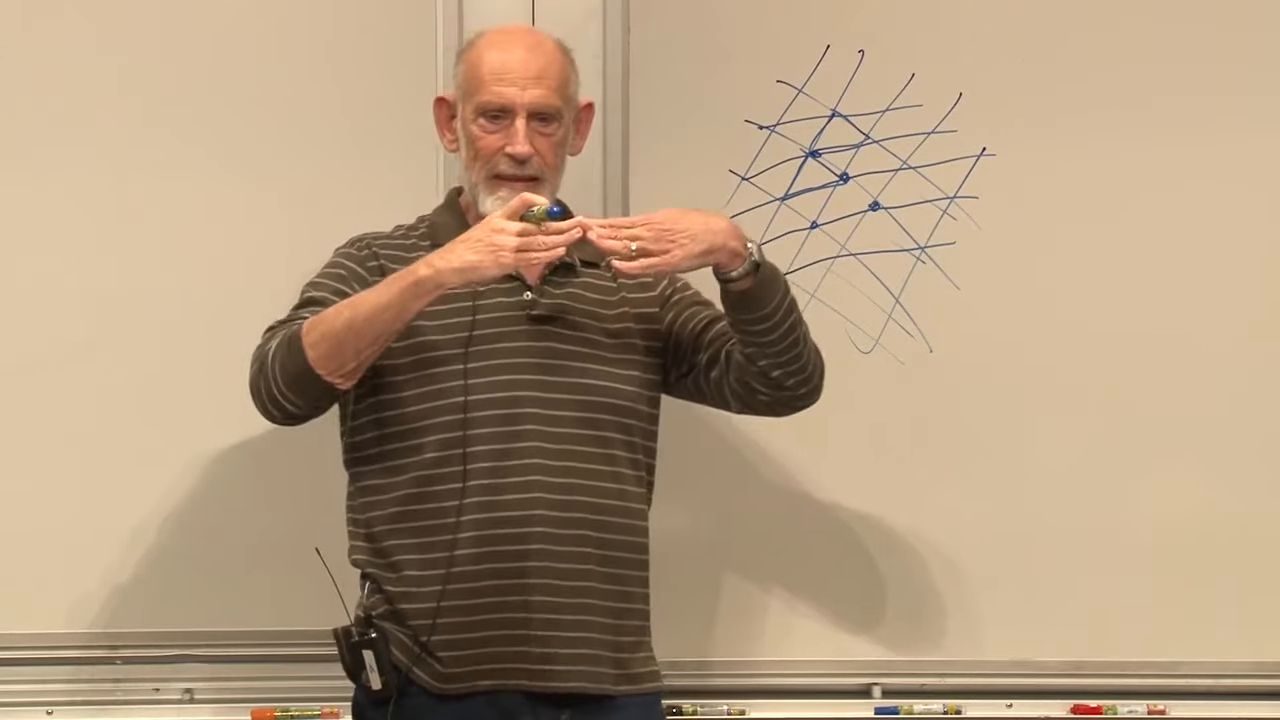
\includegraphics[width=\linewidth]{lecture_02_figure_01.png}
\caption{内蕴几何的三角形连线模型。改变一个顶点周围的连线会迫使出现一个凸包，若不改变长度就无法将其展平。}
\lectureframe{00:06:40}
\end{figure}

\begin{classroomqa}
\audiencequestion{那么，平直空间的精确定义是什么？}
\lecturerresponse{操作性的答案是：它的内蕴距离关系可以在欧几里得布局中无畸变地实现。用下文发展的语言来说，一个黎曼空间是平直的，当且仅当在所关注的整个区域内都能找到坐标，使度规为常数的克罗内克 delta。在单个点上，这总可以局部地做到；在一个区域上做到它才是非平凡的条件。曲率张量最终将陈述这一条件，而不必参照某个特殊的坐标选择。
\lecturetimestamp{00:09:15}}
\end{classroomqa}

这个答案在我们尚未有资格使用度规之前就动用了它。因此我们暂时从曲率转向张量分析。这一迂回不是可选的：必须先把度规认作张量，然后才能把它的坐标依赖性从真正的几何中分离出来。

\section{场与坐标描述}

广义相对论中的张量通常是一个张量\emph{场}：在每一点都有一个张量，其分量逐点变化。标量场是最简单的例子。曲面上的温度可以用每一点 \(P\) 处的一个数 \(S(P)\) 来表示。两个人可以用不同的坐标来标记该点，但他们必须对该处的温度取得一致。

\begin{figure}[H]
\centering
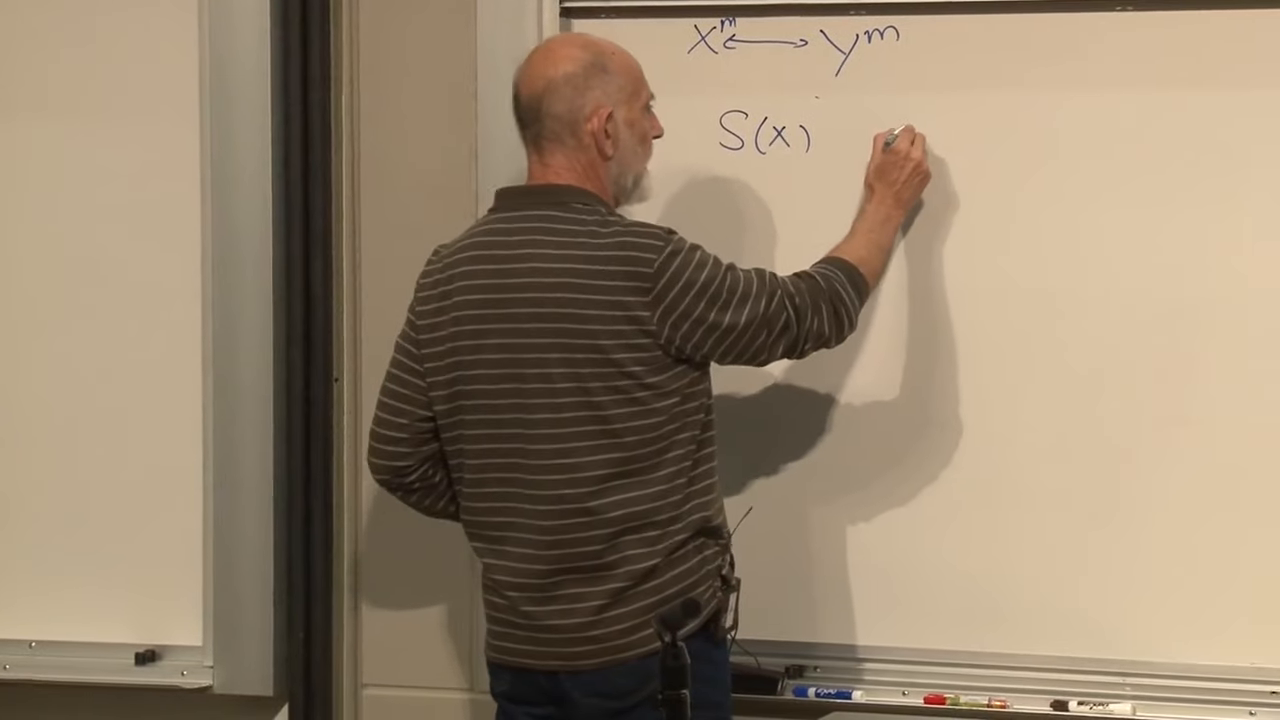
\includegraphics[width=\linewidth]{lecture_02_figure_02.png}
\caption{一个标量场，连同对同一批点的两种坐标标记。}
\lectureframe{00:11:25}
\end{figure}

设 \(x^m\) 和 \(y^m\) 是两个光滑坐标系。每一个都是从点到有序数列的映射，而在一个重叠的坐标片中，这两个数列由互逆的函数相联系，
\begin{equation}
 y^m=y^m(x^1,\ldots,x^d),
 \qquad
 x^m=x^m(y^1,\ldots,y^d).
\label{eq:coordinate-maps}
\end{equation}
光滑性允许求导，而可逆性确保不会仅仅因为改变坐标就丢失某个点，或把某个点与另一个点等同起来。

\begin{figure}[H]
\centering
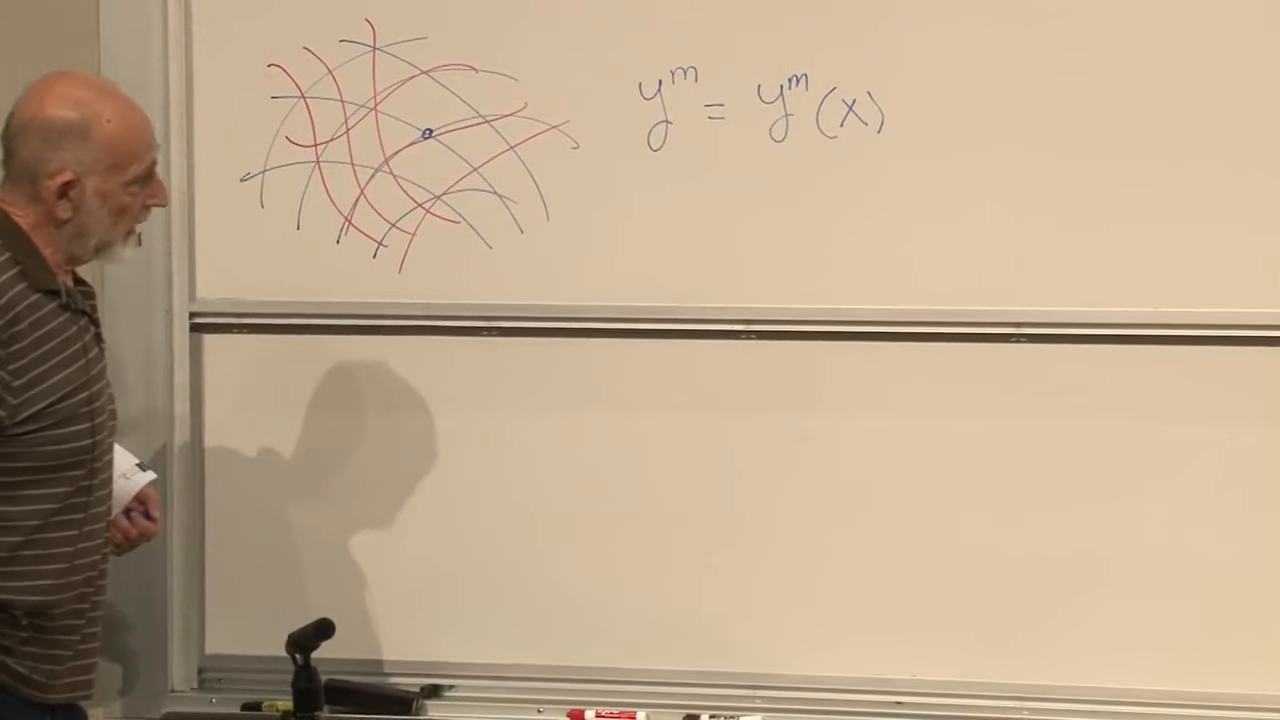
\includegraphics[width=\linewidth]{lecture_02_figure_03.png}
\caption{两个光滑、可逆的坐标映射，描述同一几何区域。}
\lectureframe{00:13:10}
\end{figure}

对于标量场，变换律简单地是
\begin{equation}
 S'(y)=S(x).
\label{eq:scalar-law}
\end{equation}
两边的函数看起来可能不同，因为它们的自变量不同，但在对应的点上它们的值一致。这是不变性陈述的原型。

\section{斜坐标与两类分量}

在用变换律定义一般张量之前，先看清为什么上、下向量指标不能当作彼此的装饰性变体，是有益的。

画一个坐标网格，其坐标轴既不垂直也未归一化。在某一点，将 \(x^m\) 增加一个坐标单位会产生一个基矢量 \(\mathbf e_m\)。用坐标语言来说，
\begin{equation}
 \mathbf e_m=\frac{\partial \mathbf r}{\partial x^m}.
\label{eq:coordinate-basis}
\end{equation}
矢量 \(\mathbf e_m\) 不必具有单位长度，也不必正交。

\begin{figure}[H]
\centering
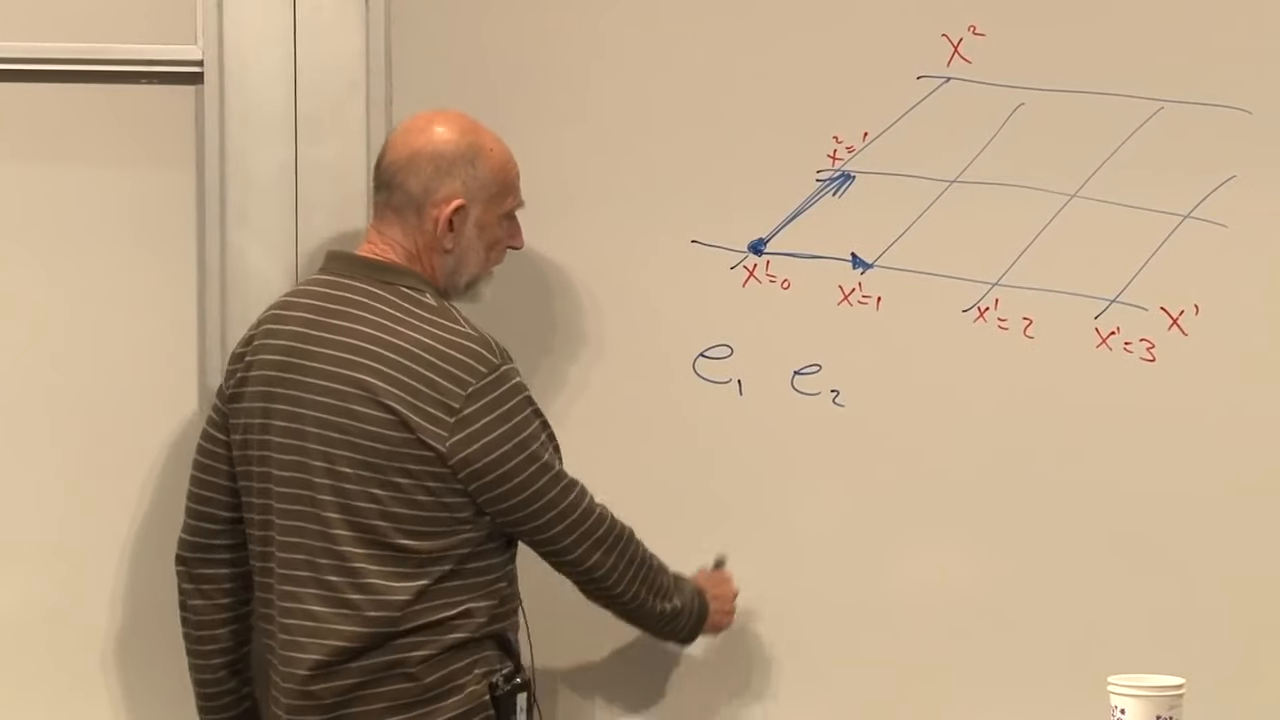
\includegraphics[width=\linewidth]{lecture_02_figure_04.png}
\caption{斜坐标网格及其坐标基矢量。}
\lectureframe{00:17:40}
\end{figure}

每个矢量 \(\mathbf V\) 都可以在这个基中展开：
\begin{equation}
 \mathbf V=V^m\mathbf e_m.
\label{eq:contravariant-expansion}
\end{equation}
这些数 \(V^m\) 就是 \emph{逆变分量}。它们是从基矢量组装出几何矢量所需的系数。

\begin{figure}[H]
\centering
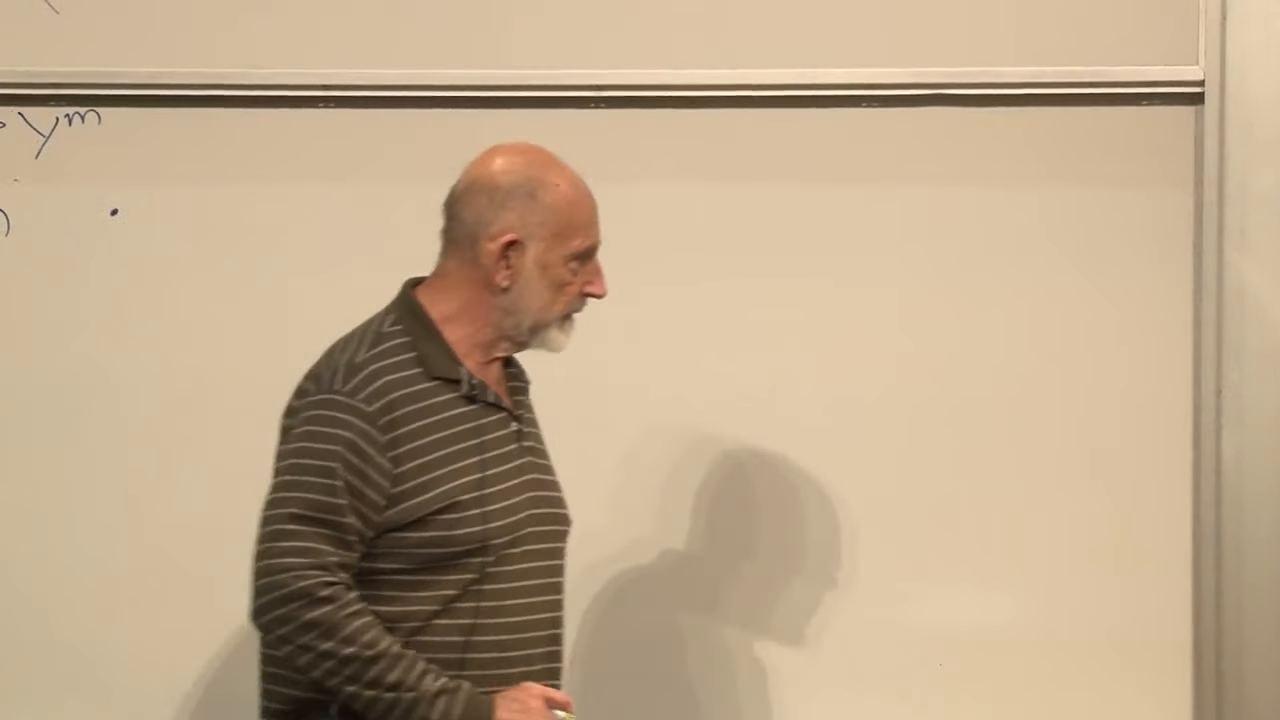
\includegraphics[width=\linewidth]{lecture_02_figure_05.png}
\caption{矢量在非正交坐标基中的展开。}
\lectureframe{00:19:20}
\end{figure}

还有另一组自然的数：
\begin{equation}
 V_m=\mathbf V\mathbin{\boldsymbol{\cdot}}\mathbf e_m.
\label{eq:covariant-projection}
\end{equation}
这些就是 \emph{协变分量}。在斜基中，它们并不只是把指标移动后的同一组系数。代入 \eqref{eq:contravariant-expansion} 得到
\begin{equation}
 V_m
 =V^n\bigl(\mathbf e_n\mathbin{\boldsymbol{\cdot}}\mathbf e_m\bigr).
\label{eq:covariant-from-basis}
\end{equation}

\begin{figure}[H]
\centering
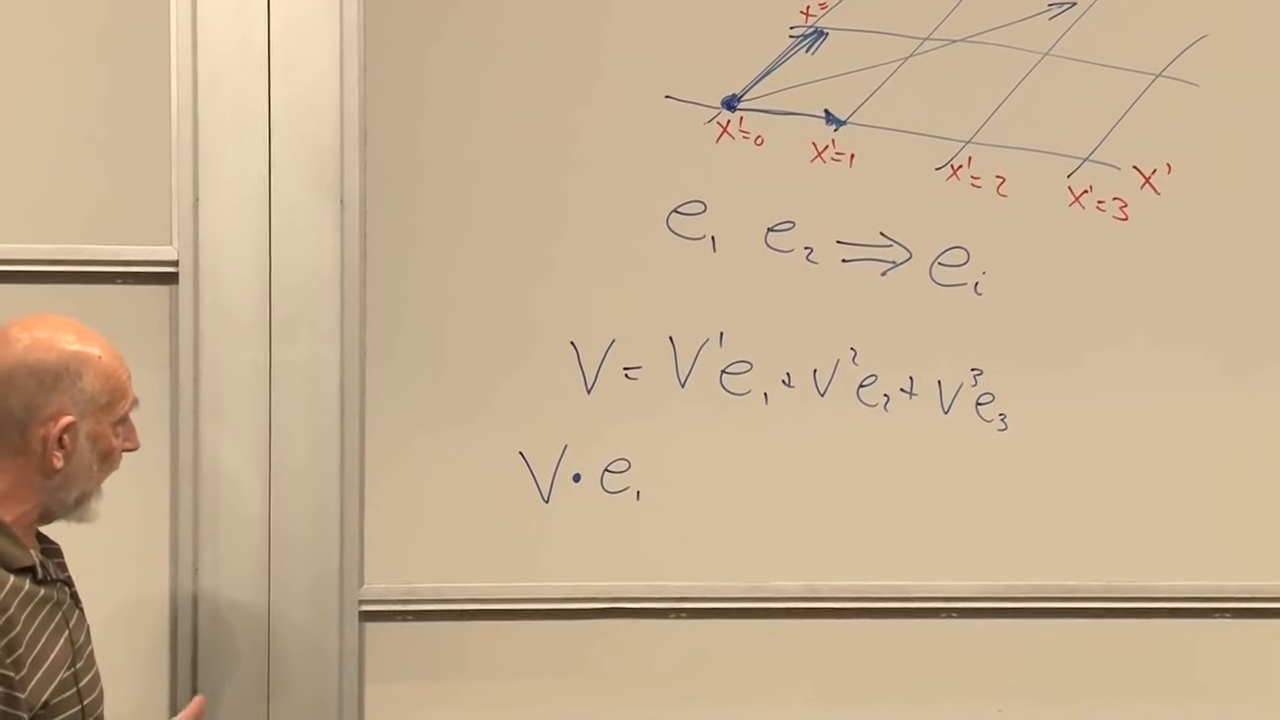
\includegraphics[width=\linewidth]{lecture_02_figure_06.png}
\caption{通过与坐标基取标量积得到的协变分量。}
\lectureframe{00:21:10}
\end{figure}

基矢量的标量积构成 Gram 矩阵
\begin{equation}
 g_{mn}=\mathbf e_m\mathbin{\boldsymbol{\cdot}}\mathbf e_n.
\label{eq:metric-gram}
\end{equation}
因此，
\begin{equation}
 V_m=g_{mn}V^n.
\label{eq:lower-vector}
\end{equation}
这是度规的首次出现。它把展开系数转换为投影，因为它同时记录了坐标基的长度和相互之间的夹角。

\begin{figure}[H]
\centering
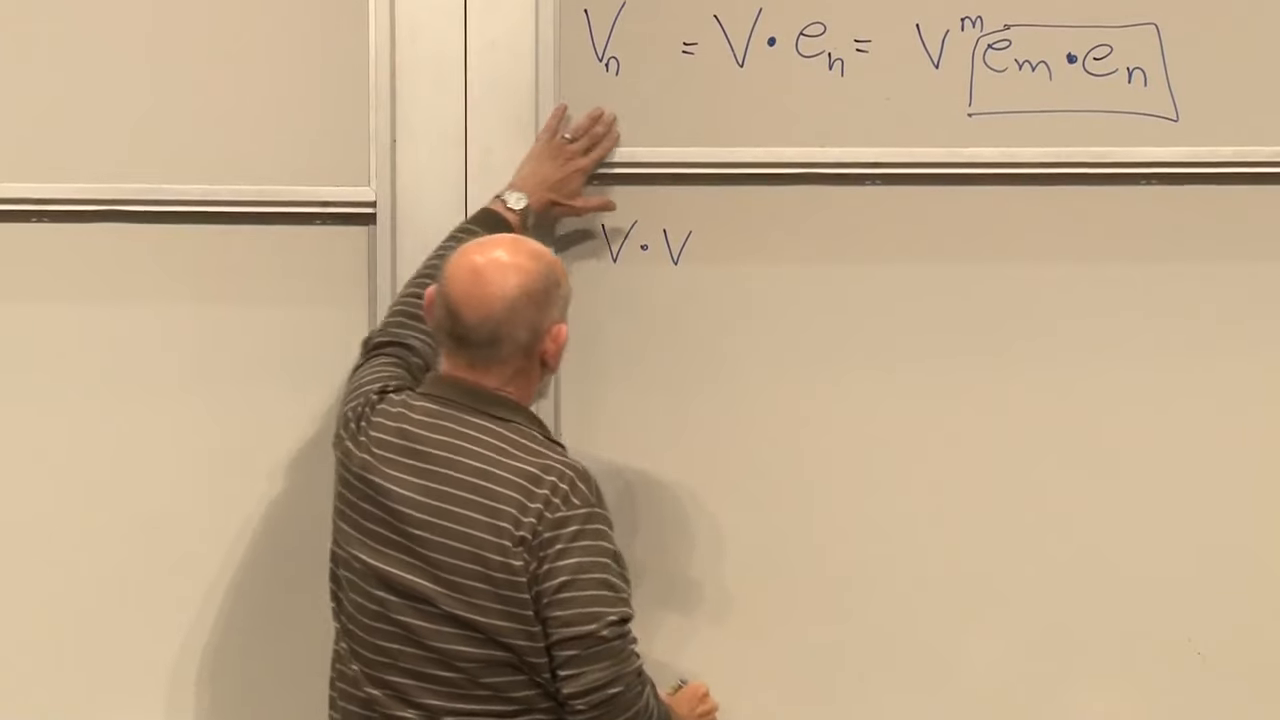
\includegraphics[width=\linewidth]{lecture_02_figure_07.png}
\caption{度规作为基矢量的 Gram 矩阵。}
\lectureframe{00:23:40}
\end{figure}

同一个矩阵也计算长度：
\begin{align}
 \mathbf V\mathbin{\boldsymbol{\cdot}}\mathbf V
 &=(V^m\mathbf e_m)\mathbin{\boldsymbol{\cdot}}
   (V^n\mathbf e_n) \notag\\
 &=g_{mn}V^mV^n.
\label{eq:vector-length}
\end{align}

\begin{figure}[H]
\centering
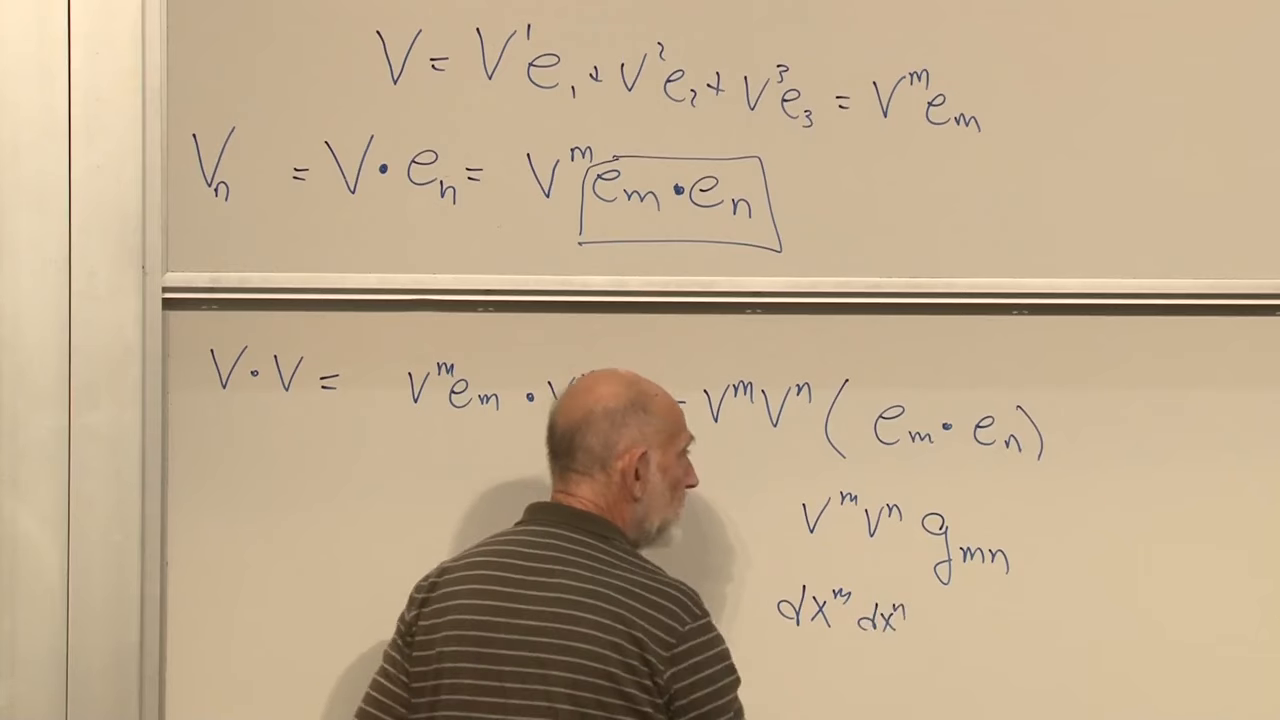
\includegraphics[width=\linewidth]{lecture_02_figure_08.png}
\caption{用度规和逆变分量写出的矢量范数。}
\lectureframe{00:25:00}
\end{figure}

\begin{classroomqa}
\audiencequestion{为什么在正式变换律之前先引入这个几何构造？}
\lecturerresponse{它赋予指标具体的含义。上指标分量是展开系数，下指标分量是对矢量的线性测量，而度规连接二者。正式定义随后将告诉我们，这些角色在任意光滑坐标变换下仍然保持。\lecturetimestamp{00:26:07}}
\end{classroomqa}

\begin{classroomqa}
\audiencequestion{协变分量和逆变分量何时具有相同的数值？}
\lecturerresponse{在正交归一的欧几里得基中，\(g_{mn}=\delta_{mn}\)，因此逐分量有 \(V_m=V^m\)。仅仅正交还不够：如果基矢量具有非单位长度，对角度规仍然会提供标度因子。
\lecturetimestamp{00:26:19}}
\end{classroomqa}

极坐标提供了一个清晰的警示。径向和角向坐标线正交相交，然而固定的变化 \(d\theta\) 对应物理距离 \(r\,d\theta\)。在平面中，
\begin{equation}
 ds^2=dr^2+r^2d\theta^2,
\label{eq:polar-metric}
\end{equation}
所以该基是正交的，但不是笛卡尔的。

\begin{figure}[H]
\centering
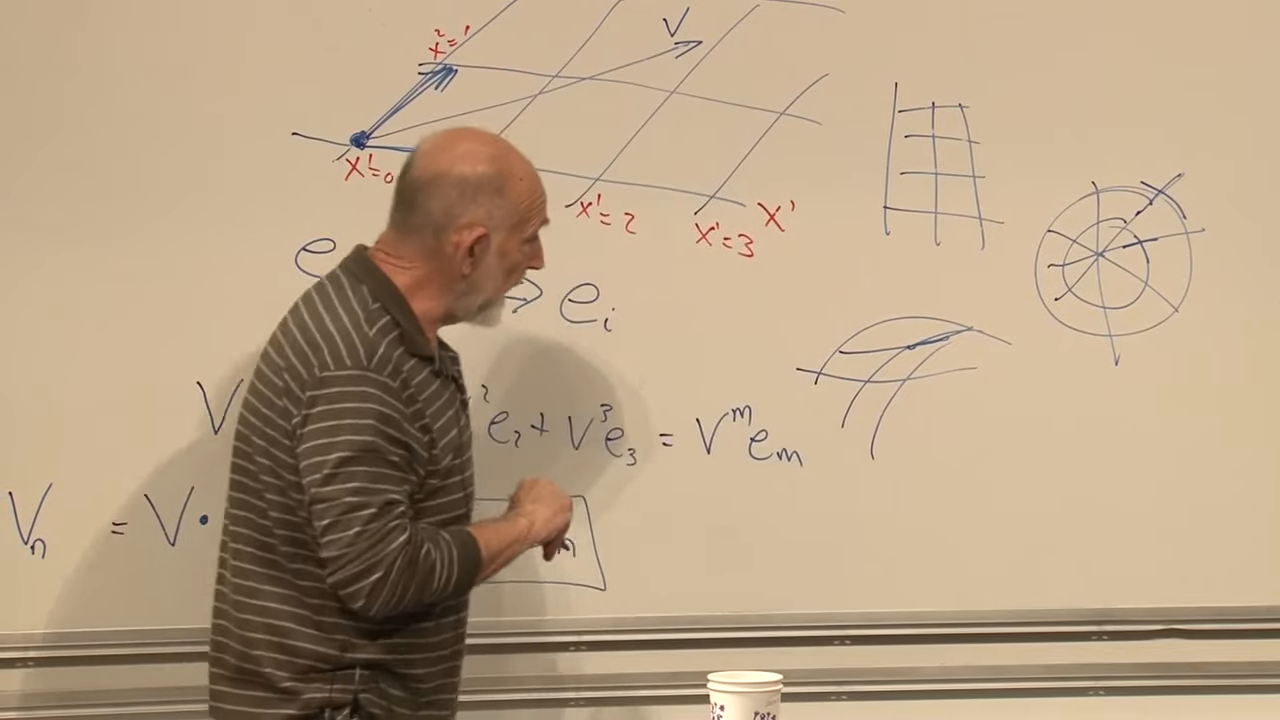
\includegraphics[width=\linewidth]{lecture_02_figure_09.png}
\caption{极坐标：正交的坐标方向，其角向标度因子随半径增大。}
\lectureframe{00:28:10}
\end{figure}

\begin{classroomqa}
\audiencequestion{协变矢量是真正不同的矢量，还是只是列出同一个矢量的第二种方式？}
\lecturerresponse{在给出度规之前，矢量与余矢量是不同类型的线性对象。矢量属于切空间；余矢量是该空间上的线性泛函。非退化度规在二者之间给出一个一一对应，由 \(V_m=g_{mn}V^n\) 表示，但不应把这种对应误认为同一。\lecturetimestamp{00:29:10}}
\end{classroomqa}

\section{变换律定义张量}

最安全的形式定义是操作性的：如果一个数组的分量按适当的雅可比因子变换，那么它就是一个张量。对 \eqref{eq:coordinate-maps} 求微分得到
\begin{equation}
 dy^m=\frac{\partial y^m}{\partial x^n}\,dx^n.
\label{eq:differential-law}
\end{equation}
任何逆变矢量都服从同一规则，
\begin{equation}
 V'^m(y)
 =\frac{\partial y^m}{\partial x^n}V^n(x).
\label{eq:contravariant-law}
\end{equation}

\begin{figure}[H]
\centering
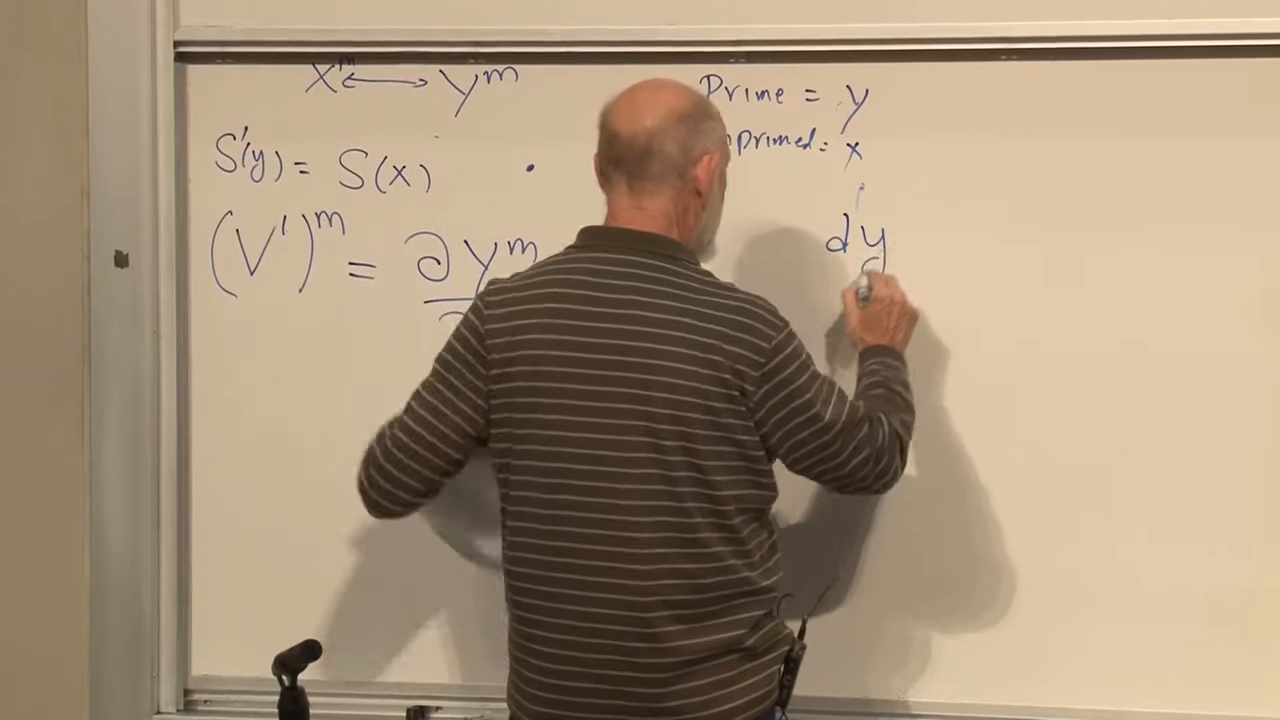
\includegraphics[width=\linewidth]{lecture_02_figure_10.png}
\caption{以坐标微分的变换为模板的逆变变换律。}
\lectureframe{00:32:50}
\end{figure}

余矢量按逆雅可比变换：
\begin{equation}
 W'_m(y)
 =\frac{\partial x^n}{\partial y^m}W_n(x).
\label{eq:covariant-law}
\end{equation}
标量的梯度是标准例子。对 \eqref{eq:scalar-law} 应用链式法则，
\begin{equation}
 \frac{\partial S}{\partial y^m}
 =\frac{\partial x^n}{\partial y^m}
  \frac{\partial S}{\partial x^n}.
\label{eq:gradient-law}
\end{equation}

\begin{figure}[H]
\centering
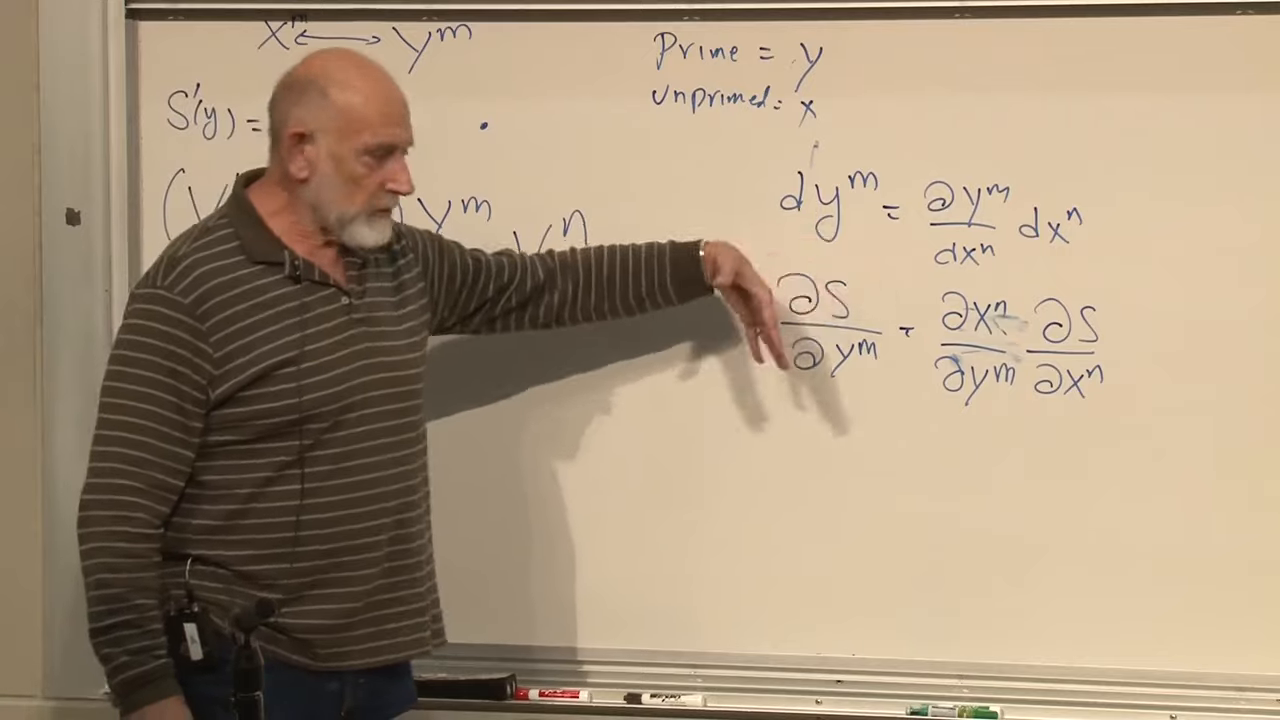
\includegraphics[width=\linewidth]{lecture_02_figure_11.png}
\caption{标量梯度按链式法则作为余矢量变换。}
\lectureframe{00:34:20}
\end{figure}

\begin{classroomqa}
\audiencequestion{上指标分量和下指标分量必然具有相同的物理单位吗？}
\lecturerresponse{不。坐标分量继承坐标及其基矢量的单位和标度约定。如果一个坐标是长度，另一个是角度，那么它们的分量甚至不必具有相同的量纲。完整的缩并才是其物理量纲与坐标无关的对象。
\lecturetimestamp{00:35:41}}
\end{classroomqa}

\begin{classroomqa}
\audiencequestion{为什么这些导数是偏导数而不是普通导数？}
\lecturerresponse{场依赖于多个坐标。雅可比矩阵所问的是，当一个自变量变化而其他自变量保持固定时，一个坐标函数如何变化，因此其元素是偏导数。\lecturetimestamp{00:36:45}}
\end{classroomqa}

这一模式现在机械地推广。每一个带上标撇的指标带来一个\(\partial y/\partial x\)因子；每一个带下标撇的指标带来一个\(\partial x/\partial y\)因子。混合张量按照
\begin{equation}
 T'^m{}_n
 =
 \frac{\partial y^m}{\partial x^p}
 \frac{\partial x^q}{\partial y^n}
 T^p{}_q,
\label{eq:mixed-law}
\end{equation}
变换，而二阶协变张量按照
\begin{equation}
 W'_{mn}
 =
 \frac{\partial x^p}{\partial y^m}
 \frac{\partial x^q}{\partial y^n}
 W_{pq}.
\label{eq:rank-two-covariant-law}
\end{equation}
变换。

\begin{figure}[H]
\centering
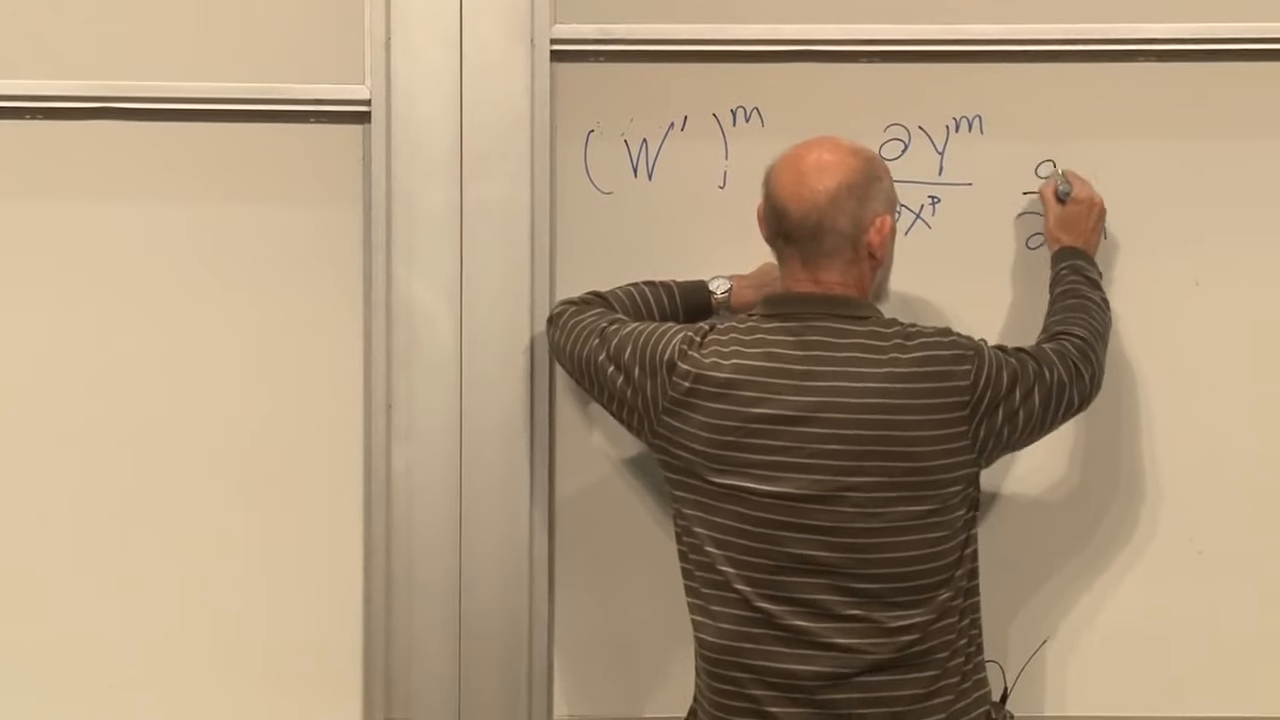
\includegraphics[width=\linewidth]{lecture_02_figure_12.png}
\caption{一个带有一个上标和一个下标的张量的变换规则。}
\lectureframe{00:40:45}
\end{figure}

\begin{figure}[H]
\centering
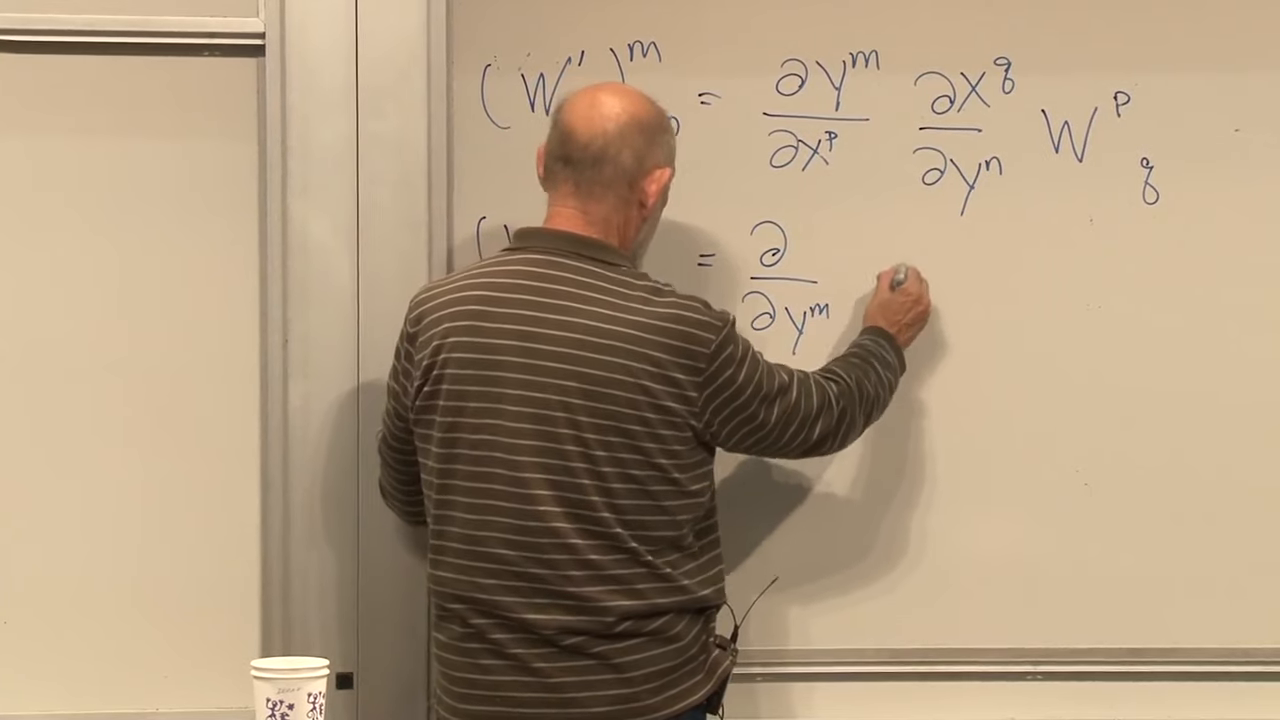
\includegraphics[width=\linewidth]{lecture_02_figure_13.png}
\caption{二阶协变变换律，每个下标对应一个逆雅可比矩阵。}
\lectureframe{00:42:15}
\end{figure}

除非另有说明，重复指标表示求和。这一约定去掉了求和号，同时保留了重建它们所需的全部信息。一个重复的哑指标在一个项中必须恰好出现两次，一次在上方，一次在下方；一个自由指标在方程的每一项中出现一次。

\begin{classroomqa}
\audiencequestion{谁引入了这种求和记号？}
\lecturerresponse{它通常被归功于爱因斯坦，因此被称为爱因斯坦求和约定。它的价值不在于历史装饰：指标模式使合法的张量运算一目了然。\lecturetimestamp{00:43:21}}
\end{classroomqa}

\section{张量方程与坐标无关的真理性}

分量随坐标变化，但张量方程在每个坐标系中都保持为真。如果两个同类型的张量满足
\(W=T\)，那么它们的差就是零张量：
\begin{equation}
 W^{m\cdots}{}_{\cdots n}
 -T^{m\cdots}{}_{\cdots n}=0.
\label{eq:tensor-equality}
\end{equation}
变换律是线性的，因此在一个坐标系中为零的分量在每个坐标系中也为零。两侧相匹配的自由指标不可或缺。不同类型对象之间的方程没有坐标无关的意义。

\begin{figure}[H]
\centering
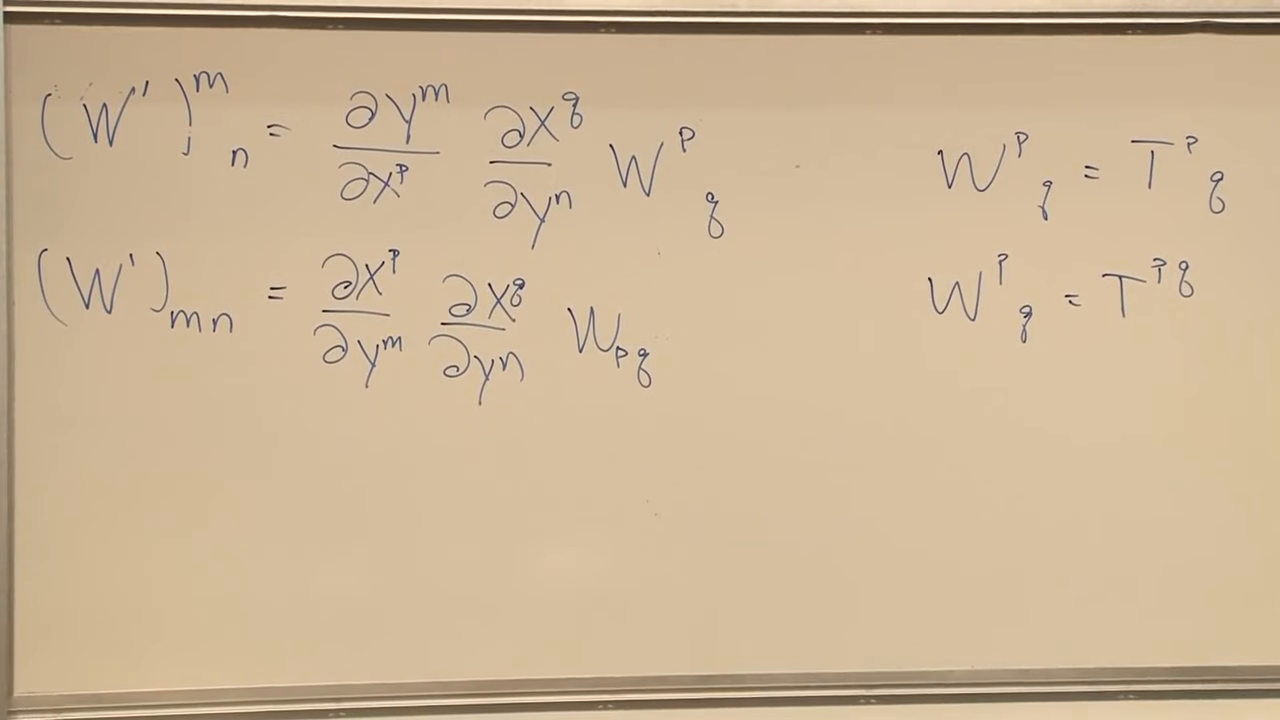
\includegraphics[width=\linewidth]{lecture_02_figure_14.png}
\caption{匹配的指标结构把分量的相等变成在每个坐标系中都成立的张量方程。}
\lectureframe{00:46:35}
\end{figure}

\begin{classroomqa}
\audiencequestion{如果矢量分量在变化，那么究竟什么是不变的？}
\lecturerresponse{几何张量以及张量方程的真理性是不变的；坐标列表则不是。标量是没有指标的特殊情形，因此它在一点处的数值在每个坐标系中都相同。\lecturetimestamp{00:47:19}}
\end{classroomqa}

\begin{classroomqa}
\audiencequestion{矢量大小是不变量的类比吗？零大小是否意味着矢量是零矢量？}
\lecturerresponse{一旦给定度规，缩并
\(g_{mn}V^mV^n\)就是一个标量，因此是不变的模平方。在正定几何中，它仅对零矢量才为零。在洛伦兹时空中，一个非零的零矢量可以具有零模，因此这两个陈述必须分开。\lecturetimestamp{00:48:04}}
\end{classroomqa}

\section{张量的允许代数运算}

黑板上汇集了将要使用的主要运算：乘以标量、同类型张量相加或相减、构成张量积、将一个上标指标与一个下标指标缩并，以及最终进行协变微分。

\begin{figure}[H]
\centering
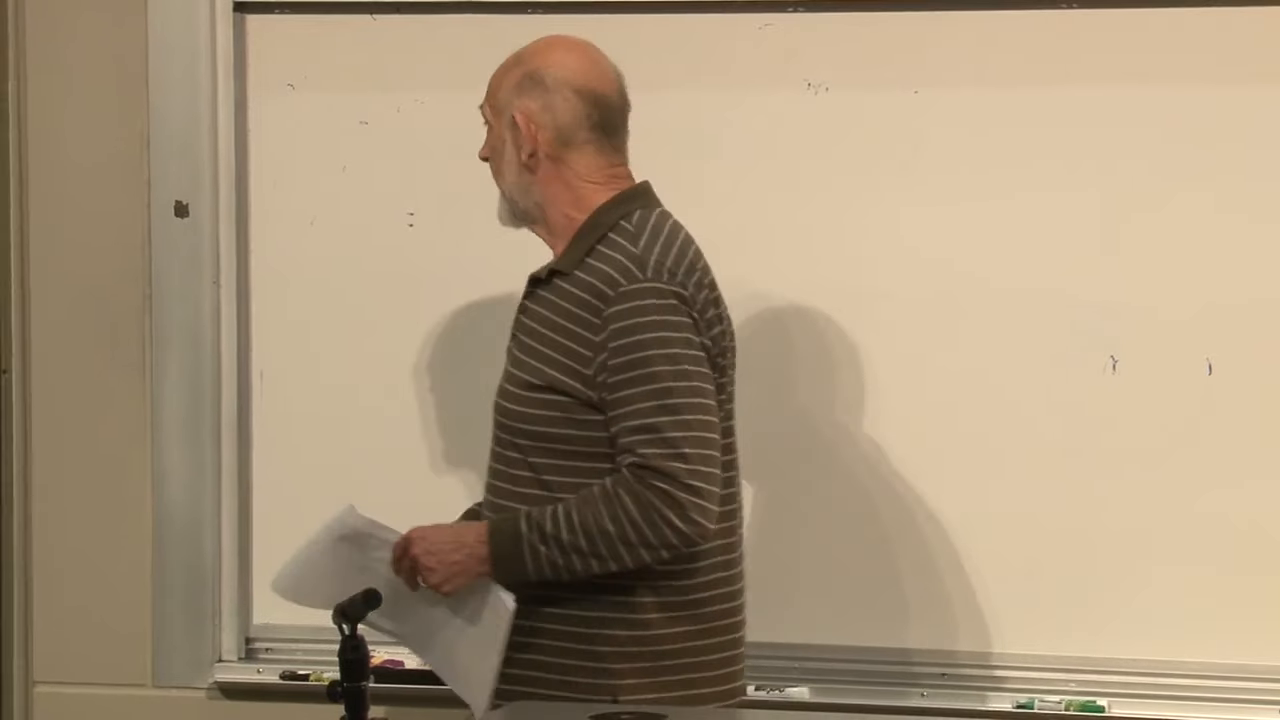
\includegraphics[width=\linewidth]{lecture_02_figure_15.png}
\caption{黑板上列出的张量运算清单：加法、乘法、缩并和微分。}
\lectureframe{00:50:40}
\end{figure}

\begin{classroomqa}
\audiencequestion{对什么求导？}
\lecturerresponse{对位置求导，因而对坐标求导。普通的成分导数一般并不像张量那样变换，因为雅可比矩阵本身也在变化。协变微分修正了这一点，但它的构造要等到几何预备知识就位之后再进行。\lecturetimestamp{00:51:49}}
\end{classroomqa}

标量乘法是直接的。加法和减法要求张量类型匹配：
\begin{equation}
 C^m{}_n=A^m{}_n+B^m{}_n,
\qquad
 D^m{}_n=A^m{}_n-B^m{}_n.
\label{eq:tensor-addition}
\end{equation}
不能把一个矢量与一个余矢量相加，也不能把一个二阶张量与一个标量相加，正如不能把一个速度与一个面积相加。

\begin{figure}[H]
\centering
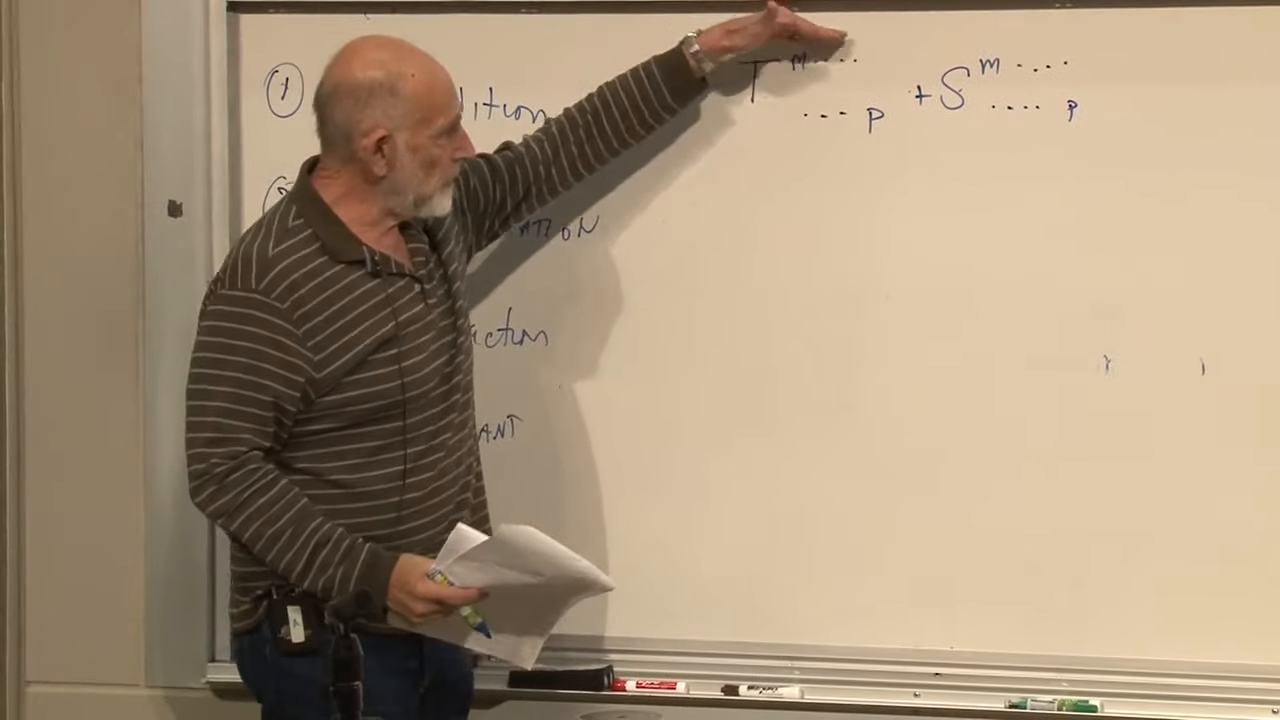
\includegraphics[width=\linewidth]{lecture_02_figure_16.png}
\caption{加法仅对具有相同自由指标模式的张量才按分量定义。}
\lectureframe{00:53:00}
\end{figure}

张量积合并其因子的所有指标。例如，
\begin{equation}
 T^{mn}=V^mW^n,
\qquad
 S^m{}_n=V^mU_n.
\label{eq:tensor-products}
\end{equation}
在四维中，\(T^{mn}\)有十六个分量。没有指标被求和，因此这是外积而不是点积。

\begin{figure}[H]
\centering
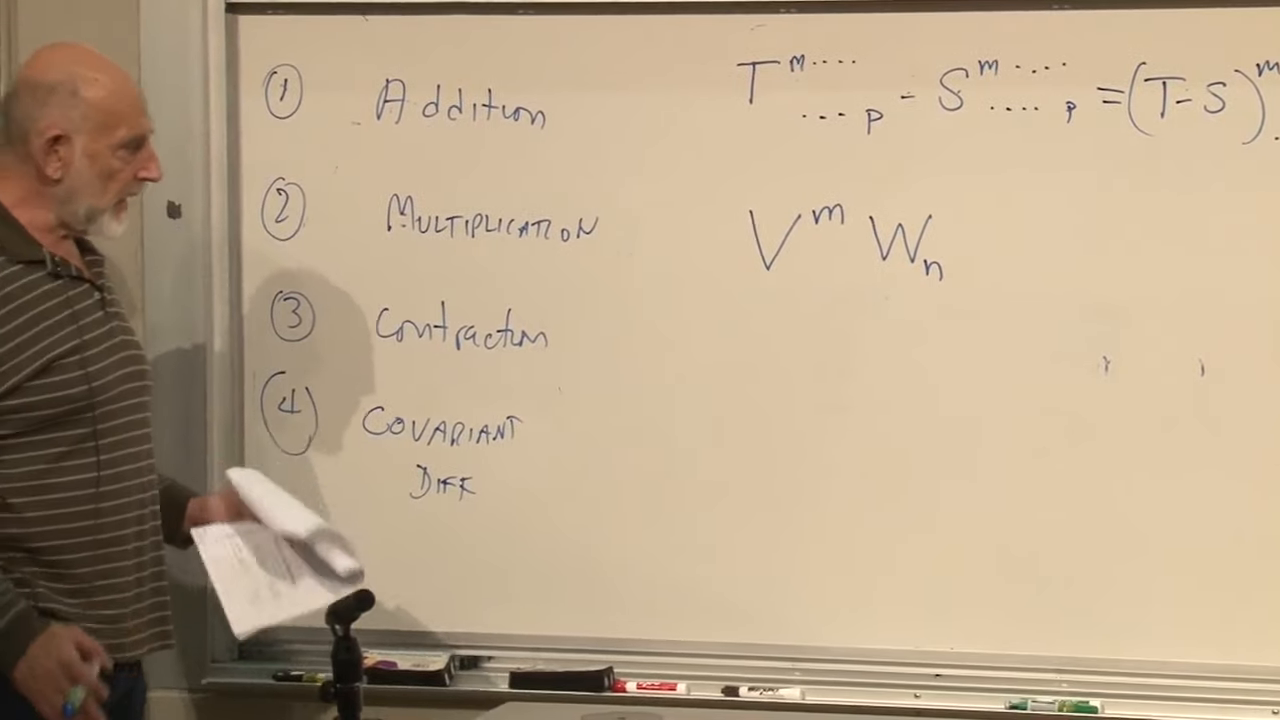
\includegraphics[width=\linewidth]{lecture_02_figure_17.png}
\caption{一个从每个矢量因子保留一个自由指标的张量积。}
\lectureframe{00:55:15}
\end{figure}

\begin{classroomqa}
\audiencequestion{这里的两个矢量相乘是点积吗？}
\lecturerresponse{不是。点积缩并一个指标并产生一个标量。张量积则让两个指标都保持自由，因此产生一个二阶张量。在四维中，那就是十六个分量，而不是一个。\lecturetimestamp{00:56:36}}
\end{classroomqa}

\begin{classroomqa}
\audiencequestion{既然分量数值可交换，交换两个矢量因子就没有区别吗？}
\lecturerresponse{对于普通的标量分量，
\(V^mW^n=W^nV^m\)。但张量的槽位是有序的。交换两个因子，然后把第一个槽位命名为\(m\)、第二个命名为\(n\)，得到的是转置后的阵列；\(T^{mn}\)未必等于\(T^{nm}\)。
\lecturetimestamp{00:58:52}}
\end{classroomqa}

\section{缩并与逆雅可比引理}

缩并的关键在于链式法则。由于坐标映射互为逆映射，
\begin{equation}
 \frac{\partial x^b}{\partial y^m}
 \frac{\partial y^m}{\partial x^a}
 =
 \frac{\partial x^b}{\partial x^a}
 =\delta^b{}_a.
\label{eq:inverse-jacobian}
\end{equation}
两个雅可比矩阵互为逆矩阵，其乘积为克罗内克{\proseunicodefont δ}。

\begin{figure}[H]
\centering
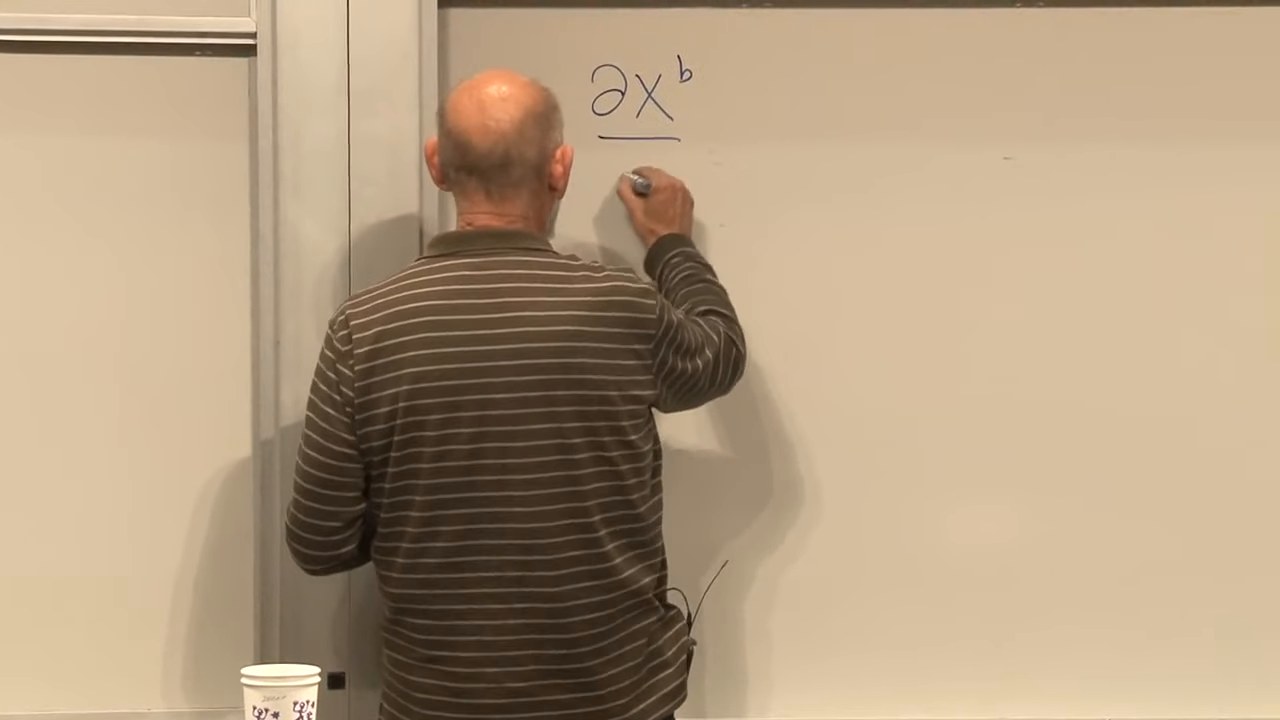
\includegraphics[width=\linewidth]{lecture_02_figure_18.png}
\caption{作为张量缩并背后引理所准备的逆雅可比恒等式。}
\lectureframe{01:02:15}
\end{figure}

\begin{classroomqa}
\audiencequestion{逆雅可比是什么样的对象？}
\lecturerresponse{它是逆坐标映射的导数矩阵。其元素为\(\partial x^b/\partial y^m\)，与\(\partial y^m/\partial x^a\)进行矩阵乘法，由多变量链式法则得到单位矩阵。\lecturetimestamp{01:02:37}}
\end{classroomqa}

一个简短的证明能让记号变得清晰。对任意标量函数\(f\)，
\begin{equation}
 \frac{\partial f}{\partial y^m}
 \frac{\partial y^m}{\partial x^a}
 =\frac{\partial f}{\partial x^a}.
\end{equation}
取\(f=x^b\)，得到
\begin{equation}
 \frac{\partial x^b}{\partial y^m}
 \frac{\partial y^m}{\partial x^a}
 =\frac{\partial x^b}{\partial x^a}
 =\delta^b{}_a.
\end{equation}

\begin{figure}[H]
\centering
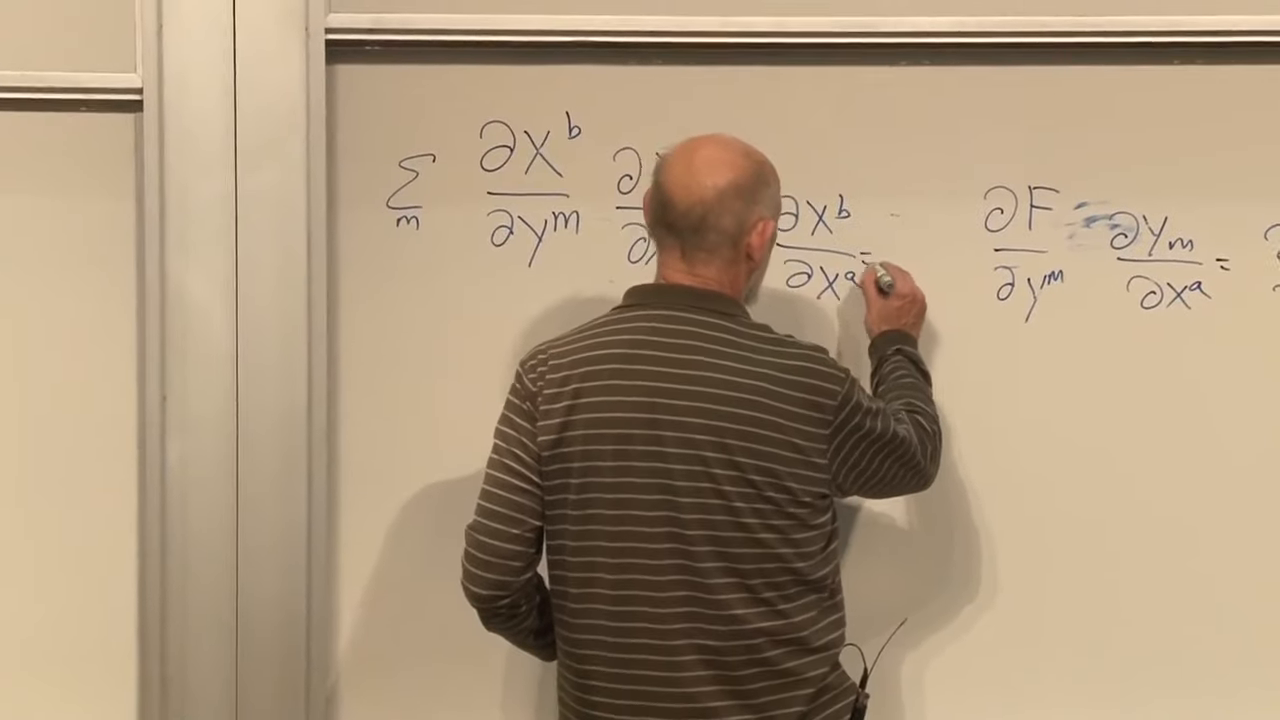
\includegraphics[width=\linewidth]{lecture_02_figure_19.png}
\caption{链式法则将逆雅可比化为克罗内克{\proseunicodefont δ}。}
\lectureframe{01:04:55}
\end{figure}

\begin{classroomqa}
\audiencequestion{\(\delta^b{}_a\)只在笛卡尔坐标中才是单位矩阵吗？}
\lecturerresponse{不是。混合张量\(\delta^b{}_a\)在每一个坐标系中都表示单位映射。写成\(\delta_{ab}\)的欧几里得度规是正交归一笛卡尔坐标所特有的，但不应把混合指标的单位张量与那个度规混为一谈。\lecturetimestamp{01:04:58}}
\end{classroomqa}

现在取一个混合张量\(T^m{}_n\)。其变换后的迹为
\begin{align}
 T'^m{}_m
 &=
 \frac{\partial y^m}{\partial x^a}
 \frac{\partial x^b}{\partial y^m}
 T^a{}_b \notag\\
 &=\delta^b{}_aT^a{}_b
 =T^a{}_a.
\label{eq:trace-invariant}
\end{align}
缩并后的量没有自由指标，因此是一个标量。

\begin{figure}[H]
\centering
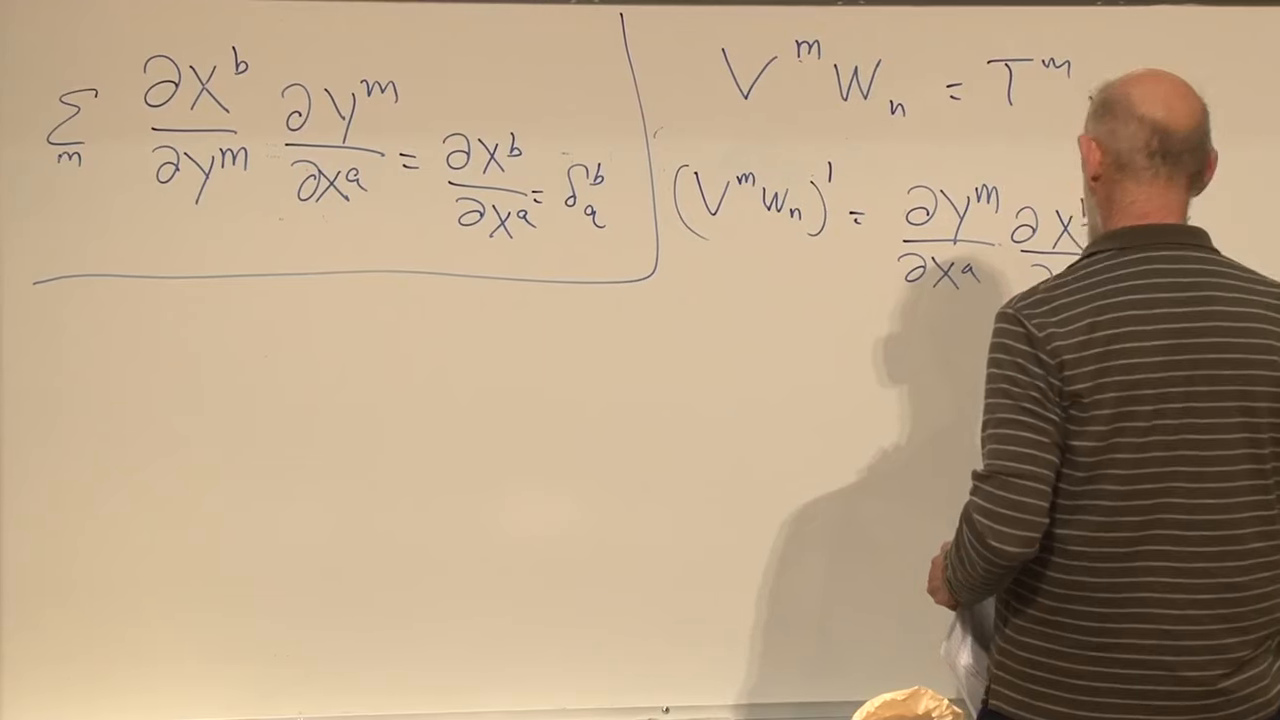
\includegraphics[width=\linewidth]{lecture_02_figure_20.png}
\caption{混合张量在上、下指标缩并之前的变换。}
\lectureframe{01:07:45}
\end{figure}

\begin{figure}[H]
\centering
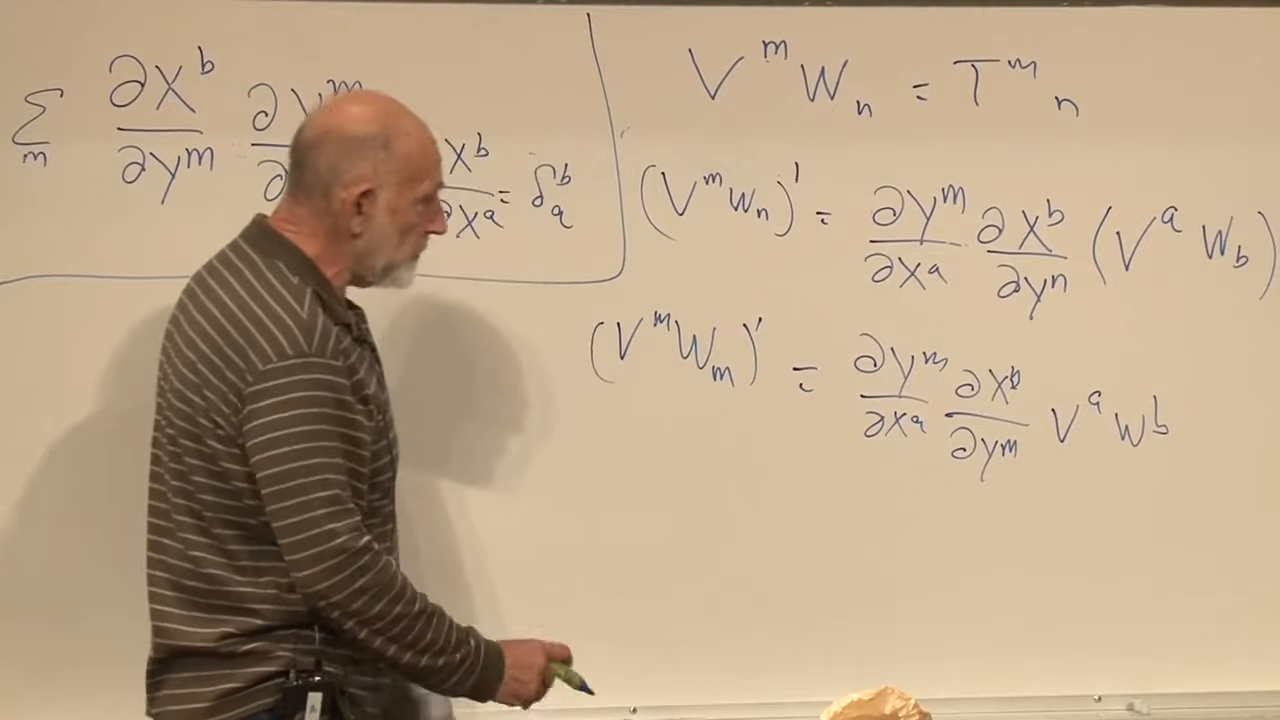
\includegraphics[width=\linewidth]{lecture_02_figure_21.png}
\caption{雅可比在缩并下相互抵消，在任一坐标系中都留下相同的标量迹。}
\lectureframe{01:10:30}
\end{figure}

\begin{classroomqa}
\audiencequestion{缩并之后，结果还带有指标吗？}
\lecturerresponse{只有被缩并的那一对消失。缩并\(T^m{}_n\)唯一的上、下指标，留下一个标量。在更高阶张量中，所有未被缩并的指标都保持自由。\lecturetimestamp{01:09:00}}
\end{classroomqa}

例如，
\begin{equation}
 A^{mn}{}_{pq}
 \longmapsto
 A^{mn}{}_{pn}
 =B^m{}_p
\label{eq:higher-rank-contraction}
\end{equation}
缩并\(n\)并使阶数降低二。具体的字母只是哑标；结构规则是，一个上槽位和一个下槽位被求和。

\begin{figure}[H]
\centering
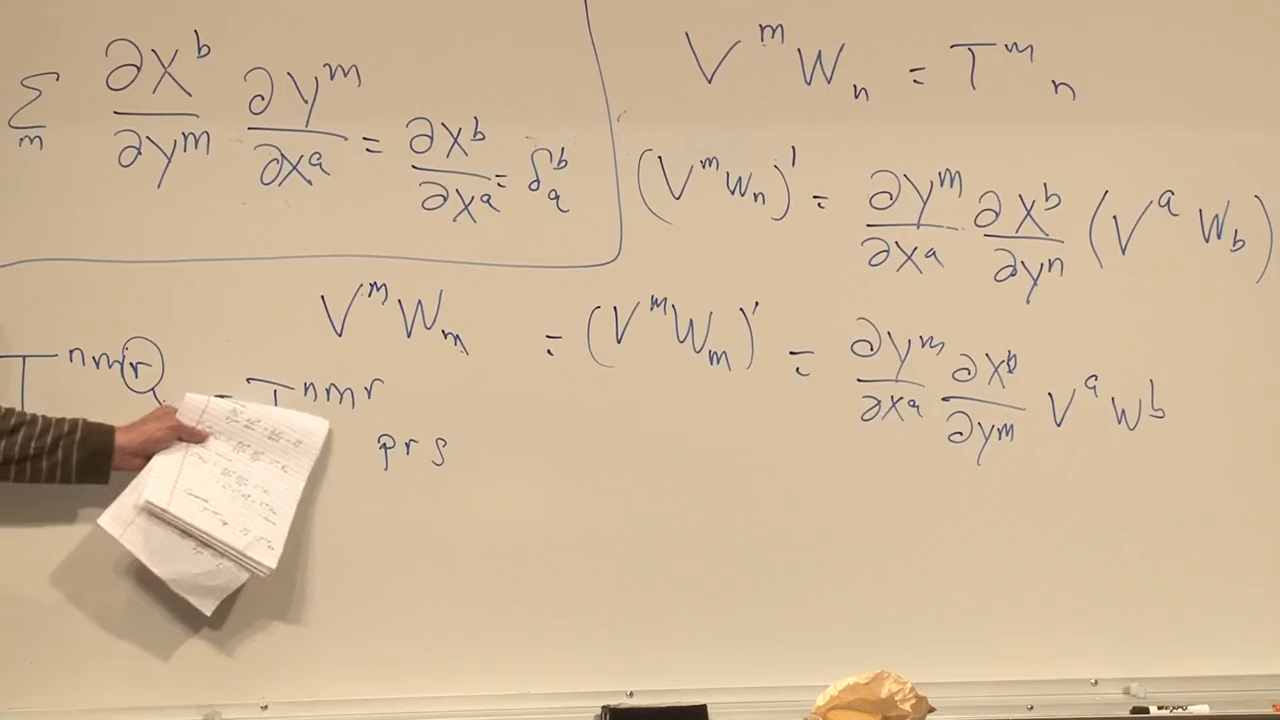
\includegraphics[width=\linewidth]{lecture_02_figure_22.png}
\caption{更高阶的缩并去掉一个上指标和一个下指标，同时保留其余自由指标。}
\lectureframe{01:12:35}
\end{figure}

\begin{classroomqa}
\audiencequestion{为什么不能以同样的方式缩并两个上指标，或两个下指标？}
\lecturerresponse{两个上指标提供两个同向的雅可比，
\(\partial y^m/\partial x^a\)和
\(\partial y^m/\partial x^b\)。它们相乘不会得到单位矩阵，因此所提出的求和没有张量变换律。可以先用度规把其中一个指标降下来，此后上--下缩并才是合法的；没有那个额外的张量，该运算就不是坐标不变的。\lecturetimestamp{01:13:03}}
\end{classroomqa}

\begin{figure}[H]
\centering
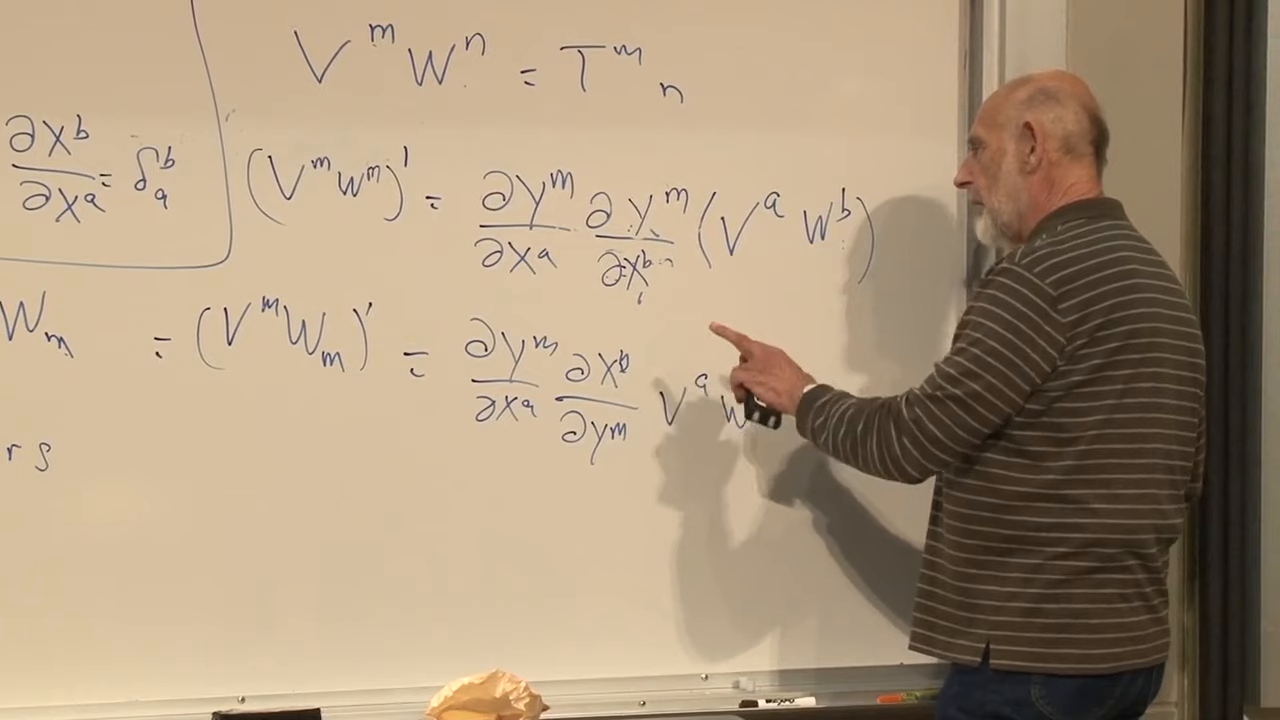
\includegraphics[width=\linewidth]{lecture_02_figure_23.png}
\caption{所尝试的同变型缩并留下两个同向的雅可比，因此不会化为单位矩阵。}
\lectureframe{01:14:30}
\end{figure}

\begin{classroomqa}
\audiencequestion{缩并是张量版本的内积吗？}
\lecturerresponse{缩并把一个矢量槽位与一个余矢量槽位配对，是基本的配对不变量。有了度规，两个矢量可以变成这样一对，所以熟悉的内积就是先用度规再缩并。\lecturetimestamp{01:14:43}}
\end{classroomqa}

\begin{classroomqa}
\audiencequestion{被缩并的两个指标必须在同一范围内取值吗？}
\lecturerresponse{是的。它们指的是同一个\(d\)维切空间与余切空间的对偶基。否则求和与逆雅可比恒等式就无法定义。\lecturetimestamp{01:15:13}}
\end{classroomqa}

\begin{classroomqa}
\audiencequestion{为什么一个在某个参考系中为零的张量会在每个参考系中都为零？}
\lecturerresponse{每个变换后的分量都是原始分量的线性组合。当所有输入分量都为零时，所有这些组合都为零。正是这种简单的线性性使张量方程与坐标无关。\lecturetimestamp{01:15:31}}
\end{classroomqa}

\section{由平方距离得到的度规}

现在回到几何。对于分量为 \(dx^m\) 的无穷小位移，用下式定义其平方长度
\begin{equation}
 ds^2=g_{mn}(x)\,dx^m dx^n.
\label{eq:line-element}
\end{equation}
这就是广义勾股定理。度规可以逐点变化，而非对角项记录了坐标方向的不正交性。

\begin{figure}[H]
\centering
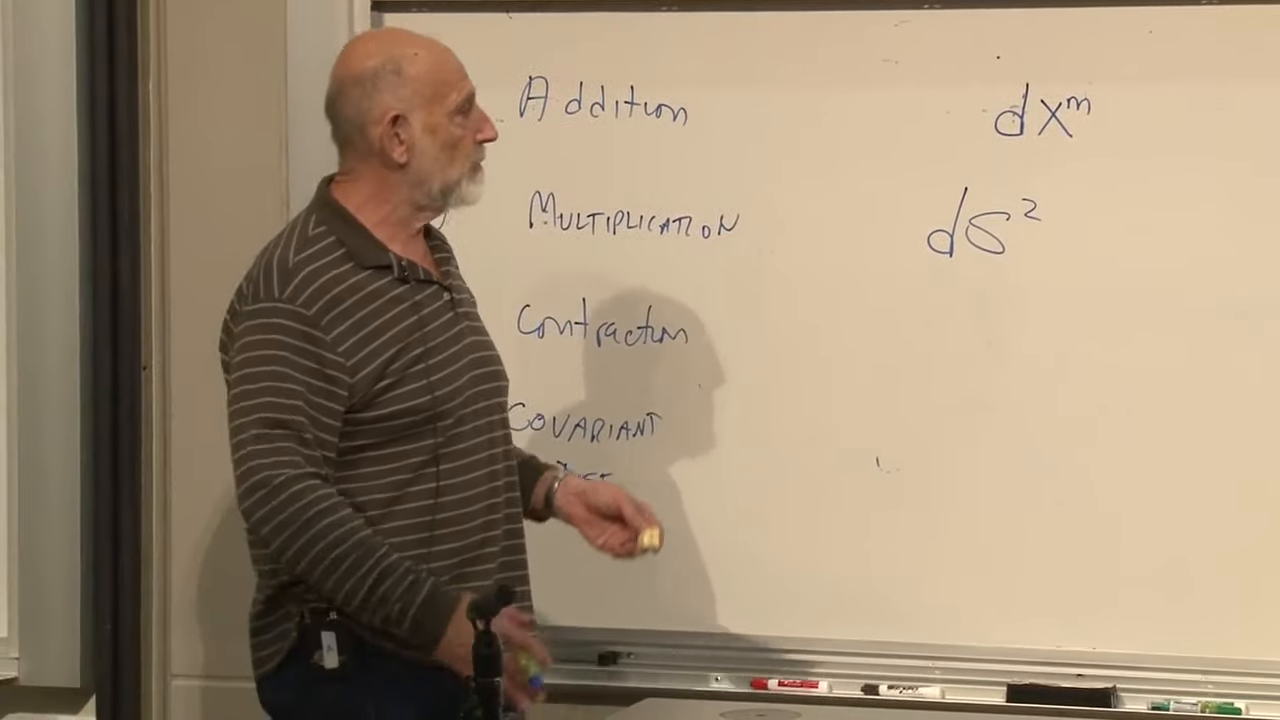
\includegraphics[width=\linewidth]{lecture_02_figure_24.png}
\caption{张量运算的清单让位于无穷小线元的二次定义。}
\lectureframe{01:18:45}
\end{figure}

只有对称部分有贡献，因为
\(dx^m dx^n=dx^n dx^m\)。因此我们可以取
\begin{equation}
 g_{mn}=g_{nm}.
\label{eq:metric-symmetry}
\end{equation}
在 \(d\) 维中，对称度规有
\begin{equation}
 \frac{d(d+1)}{2}
\label{eq:metric-component-count}
\end{equation}
个独立分量：四维中十个，三维中六个，二维中三个。

\begin{figure}[H]
\centering
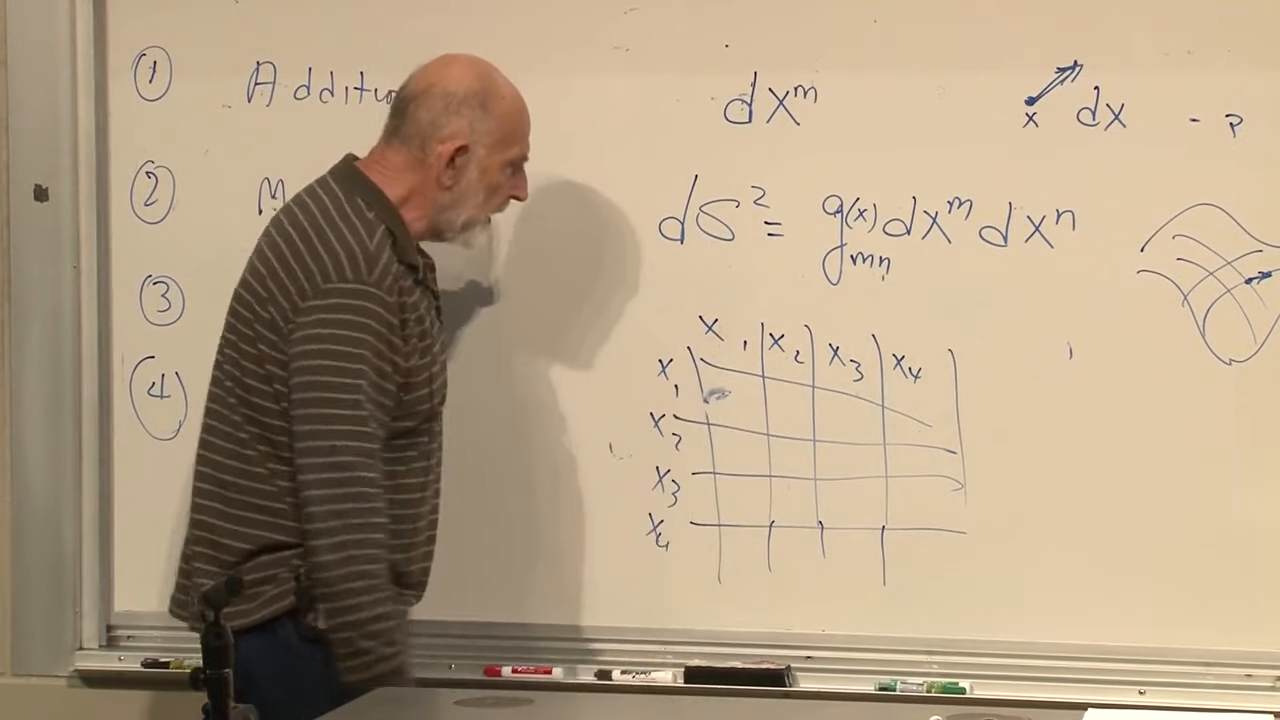
\includegraphics[width=\linewidth]{lecture_02_figure_25.png}
\caption{线元以及用于计数度规独立分量的对称分量阵列。}
\lectureframe{01:21:35}
\end{figure}

\begin{classroomqa}
\audiencequestion{为什么四维中有十个独立的度规分量，而不是十六个？}
\lecturerresponse{有四个对角项和六个无序的非对角对。等价地，
\(4(4+1)/2=10\)。反对称部分会乘以对称乘积 \(dx^m dx^n\) 并抵消。\lecturetimestamp{01:19:50}}
\end{classroomqa}

\begin{classroomqa}
\audiencequestion{三维中有多少个独立分量？}
\lecturerresponse{六个：三个对角项和三个非对角对，即 \(3(3+1)/2\)。\lecturetimestamp{01:20:47}}
\end{classroomqa}

\begin{classroomqa}
\audiencequestion{那二维中呢？}
\lecturerresponse{三个：\(g_{11}\)、\(g_{22}\)，以及唯一的对称对 \(g_{12}=g_{21}\)。\lecturetimestamp{01:22:28}}
\end{classroomqa}

\subsection{为什么度规是张量}

平方距离是标量。因此用两个坐标系写出同一个位移给出
\begin{equation}
 g_{mn}(x)\,dx^m dx^n
 =
 g'_{pq}(y)\,dy^pdy^q.
\label{eq:length-invariance}
\end{equation}
使用
\begin{equation}
 dx^m=\frac{\partial x^m}{\partial y^p}\,dy^p
\end{equation}
两次：
\begin{align}
 ds^2
 &=
 g_{mn}(x)
 \frac{\partial x^m}{\partial y^p}
 \frac{\partial x^n}{\partial y^q}
 dy^pdy^q.
\label{eq:metric-transform-derivation}
\end{align}
与带撇表达式的比较确定
\begin{equation}
 g'_{pq}(y)
 =
 \frac{\partial x^m}{\partial y^p}
 \frac{\partial x^n}{\partial y^q}
 g_{mn}(x).
\label{eq:metric-transformation}
\end{equation}
这正是协变二阶张量的变换律。

\begin{figure}[H]
\centering
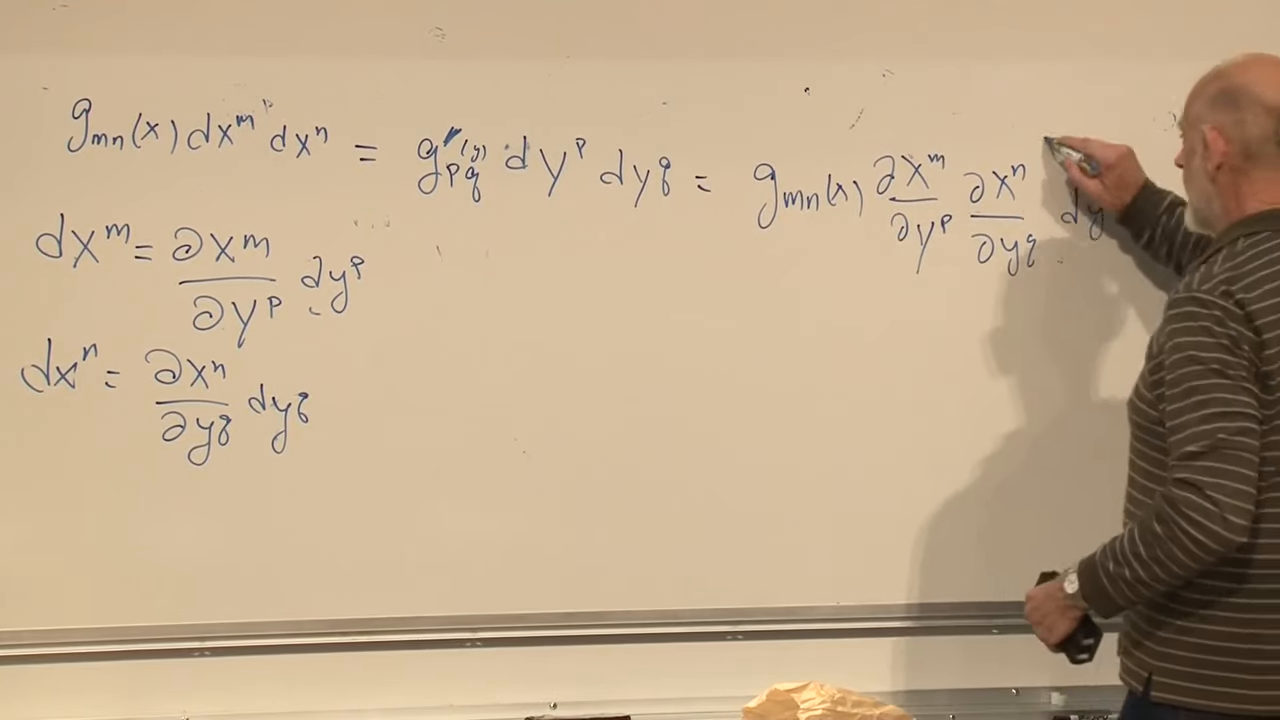
\includegraphics[width=\linewidth]{lecture_02_figure_26.png}
\caption{由标量线元的不变性推导度规变换律。}
\lectureframe{01:26:25}
\end{figure}

这一结论也解释了为什么有两个下指标。度规的每个下指标与位移分量携带的一个上指标配对。在坐标变换下，\eqref{eq:metric-transformation} 中的两个逆雅可比抵消微分的两个正雅可比，使 \(ds^2\) 保持不变。

\section{度规矩阵及其逆}

在一点处，\(g_{mn}\) 是一个对称矩阵：
\begin{equation}
 [g_{mn}]
 =
 \begin{pmatrix}
 g_{11} & g_{12} & \cdots \\
 g_{12} & g_{22} & \cdots \\
 \vdots & \vdots & \ddots
 \end{pmatrix}.
\label{eq:metric-matrix}
\end{equation}

\begin{figure}[H]
\centering
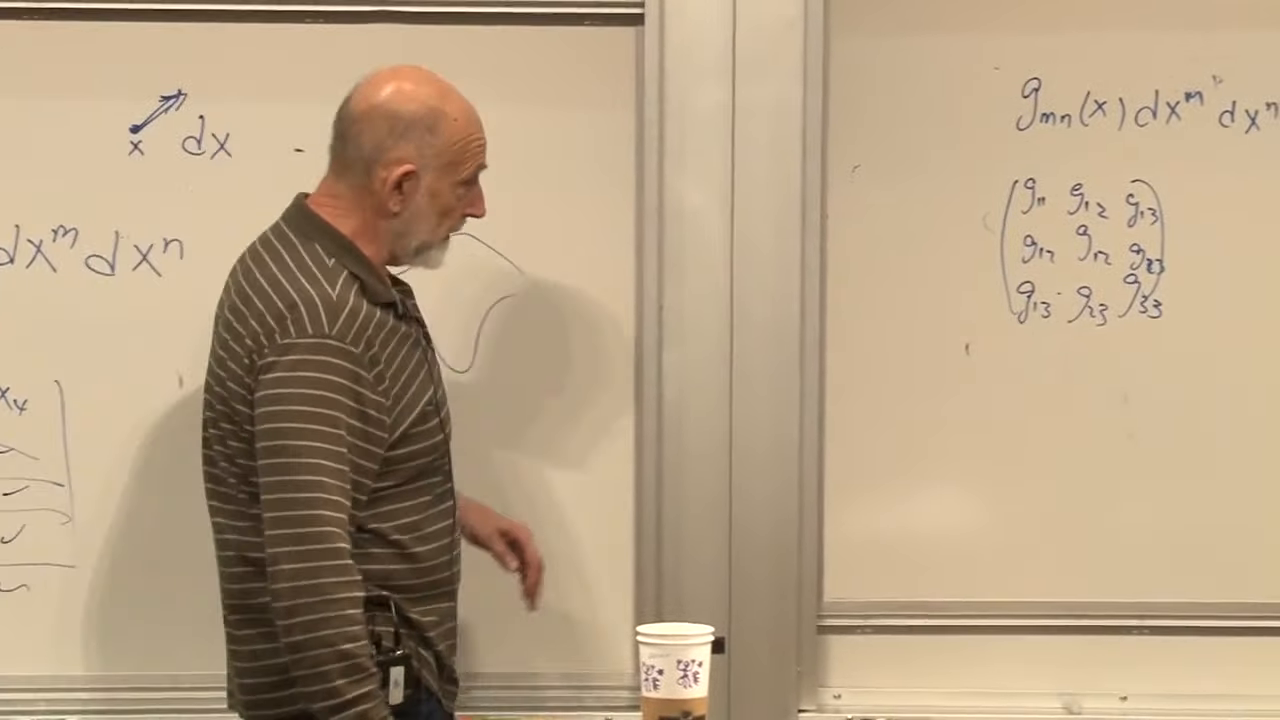
\includegraphics[width=\linewidth]{lecture_02_figure_27.png}
\caption{在度规的张量变换律建立之后，将其表示为对称矩阵。}
\lectureframe{01:28:50}
\end{figure}

度规要求是非退化的：它没有零特征值，因此拥有逆。将该逆记为 \(g^{mn}\)。用指标记号表示，
\begin{equation}
 g_{mn}g^{np}=\delta_m{}^p.
\label{eq:inverse-metric}
\end{equation}
重复的 \(n\) 被求和，而 \(m\) 和 \(p\) 标记乘积的行和列。

\begin{figure}[H]
\centering
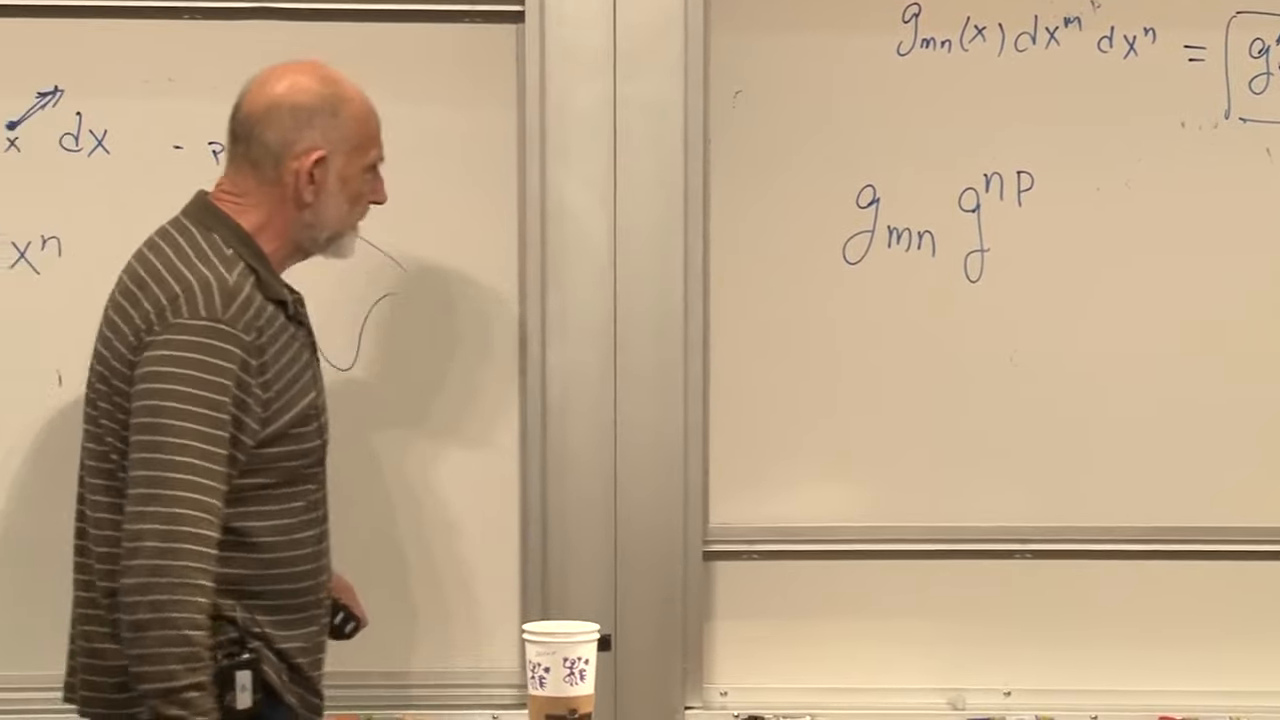
\includegraphics[width=\linewidth]{lecture_02_figure_28.png}
\caption{通过 \(g_{mn}g^{np}=\delta_m{}^p\) 引入的逆度规。}
\lectureframe{01:31:40}
\end{figure}

\begin{classroomqa}
\audiencequestion{一点处的向量和张量实际上生活在哪里？}
\lecturerresponse{一点处的向量构成其切空间 \(T_P M\)；余向量构成对偶空间 \(T_P^*M\)。更高阶张量属于这些空间的张量积。张量场将这样的对象光滑地赋予每一点。度规是切空间上的双线性形式，其逆是余切空间上相应的双线性形式。\lecturetimestamp{01:34:15}}
\end{classroomqa}

\begin{figure}[H]
\centering
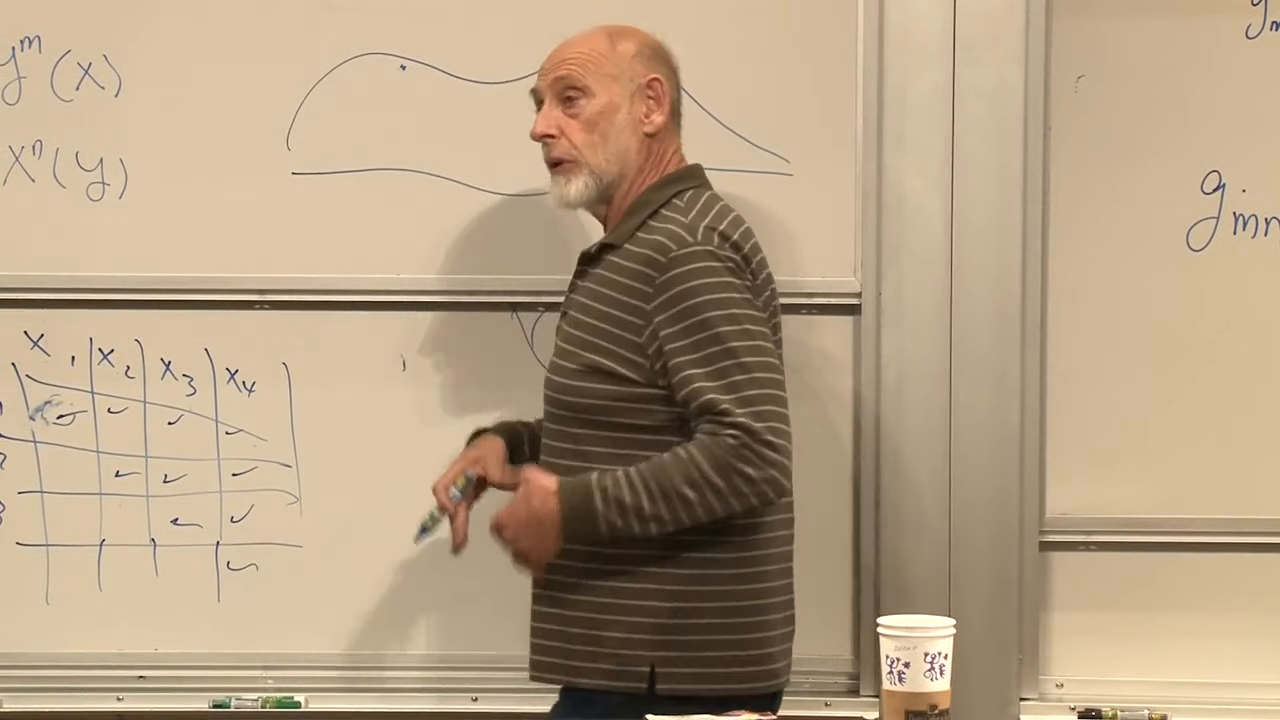
\includegraphics[width=\linewidth]{lecture_02_figure_29.png}
\caption{在弯曲流形某一点处的切空间中画出的向量。}
\lectureframe{01:35:45}
\end{figure}

\begin{classroomqa}
\audiencequestion{
\(g_{mn}g^{np}=\delta_m{}^p\) 是否只指 \(m=p\) 的情形？}
\lecturerresponse{不。它是完整的矩阵方程。对于每个有序对 \((m,p)\)，当 \(m=p\) 时求和乘积为一，当 \(m\ne p\) 时为零。所有对角和非对角方程同时成立。\lecturetimestamp{01:36:50}}
\end{classroomqa}

\begin{figure}[H]
\centering
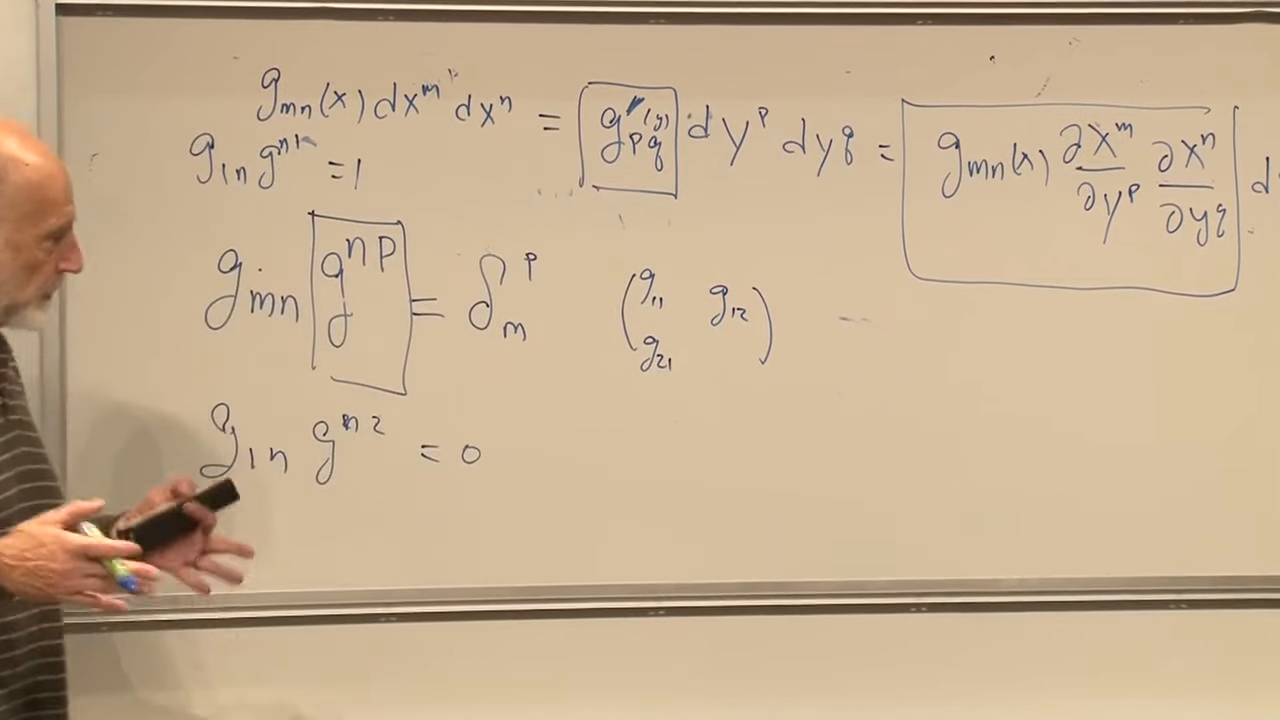
\includegraphics[width=\linewidth]{lecture_02_figure_30.png}
\caption{将逆关系解释为完整的混合指标单位矩阵。}
\lectureframe{01:38:50}
\end{figure}

在二维中这意味着
\begin{equation}
 \begin{pmatrix}
 g_{11} & g_{12}\\
 g_{12} & g_{22}
 \end{pmatrix}
 \begin{pmatrix}
 g^{11} & g^{12}\\
 g^{12} & g^{22}
 \end{pmatrix}
 =
 \begin{pmatrix}
 1&0\\
 0&1
 \end{pmatrix}.
\label{eq:two-dimensional-inverse}
\end{equation}
例如，
\begin{align}
 g_{11}g^{11}+g_{12}g^{12}&=1,\\
 g_{11}g^{12}+g_{12}g^{22}&=0.
\end{align}
另一行给出其余两个方程。

\begin{figure}[H]
\centering
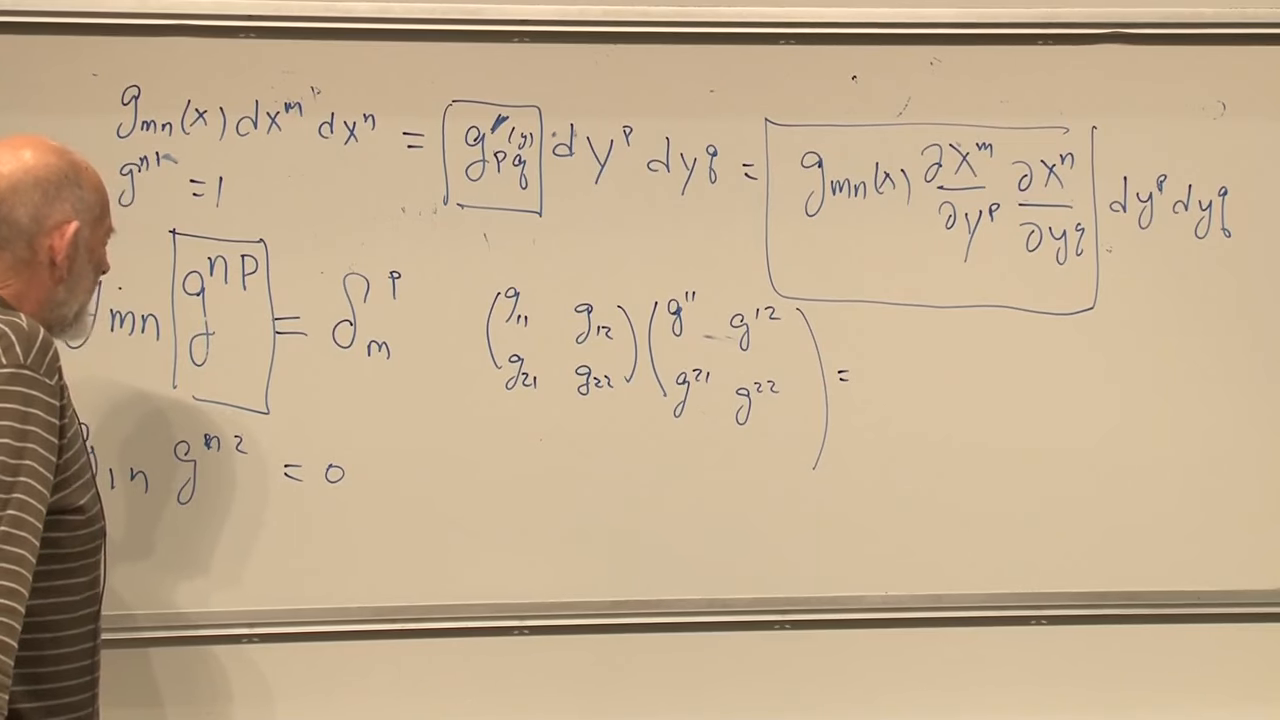
\includegraphics[width=\linewidth]{lecture_02_figure_31.png}
\caption{逆度规恒等式展开为显式的二维矩阵乘积。}
\lectureframe{01:40:00}
\end{figure}

\begin{classroomqa}
\audiencequestion{度规必须是正定的吗？}
\lecturerresponse{对于通常的黎曼几何，正定性使每个非零长度的平方都为正。而时空改用洛伦兹度规，其中一个符号与另外三个相反。这里两种情形所要求的都是非退化性，而非正定性。
\lecturetimestamp{01:42:18}}
\end{classroomqa}

\begin{classroomqa}
\audiencequestion{为什么要排除零特征值？}
\lecturerresponse{零特征值会使度规矩阵奇异，因此\(g^{mn}\)不存在，度规也就无法在矢量与余矢量之间建立一一对应。在通常的微分几何意义下，度规必须是非退化的。\lecturetimestamp{01:43:56}}
\end{classroomqa}

\begin{classroomqa}
\audiencequestion{四维度规的十个独立分量与十维弦论有什么关系吗？}
\lecturerresponse{没有。前一个十不过是\(4(4+1)/2\)，即一个对称四乘四矩阵的条目数。超弦理论中十个时空维度的出现则有不同的来源。\lecturetimestamp{01:44:32}}
\end{classroomqa}

\begin{classroomqa}
\audiencequestion{如果洛伦兹时空存在长度为零的非零矢量，这是否使度规不可逆？}
\lecturerresponse{不会。零矢量满足\(g_{mn}V^mV^n=0\)，这是不定二次型内部的一种抵消。它并不是满足\(g_{mn}V^n=0\)的零特征值矢量。例如，闵可夫斯基度规的特征值为\(\pm1\)，它完全可逆，同时仍容许类光矢量。\lecturetimestamp{01:45:02}}
\end{classroomqa}

\section{接下来是什么}

现在我们可以清晰地陈述这一几何纲领了。度规记录无穷小距离，协变地变换，并且具有逆。它的分量之所以可能显得复杂，仅仅是因为坐标复杂。要判断几何本身是否弯曲，我们必须以与坐标无关的方式比较邻近点处的度规。

普通导数是不够的，因为对张量求导时，也会对其变换律中依赖于位置的雅可比行列式求导。因此下一步是协变微分。由度规的导数可以构造联络；由该联络的导数与乘积可以构造曲率。只有到那时，卷曲书页的问题才会得到最终的、内禀的答案。
